\documentclass[aspectratio=43]{beamer}

\usepackage[ngerman]{babel}
\usepackage[utf8]{inputenc}
\usepackage[absolute,overlay]{textpos}
\usepackage{xcolor}

\definecolor{black}{HTML}{3C3C3C}
\definecolor{green}{HTML}{BBE08C}

\mode<presentation>
{
  \usetheme[compress]{Torino}
}

\newcommand{\concept}[2]{
  \begin{block}{#1}
    \pause
    #2
  \end{block}
}

\newcommand{\pattern}[2]{
  \begin{alertblock}{Problem}
    #1
  \end{alertblock}
  \pause
  \begin{exampleblock}{Lösung}
    #2
  \end{exampleblock}
}

\newcommand{\boxx}[1]{
  \colorbox{black}{
    \color{green}{#1}
  }
}

\newcommand{\photoby}[3]{
  \begin{textblock*}{\paperwidth}[0.25,0](\textwidth,\textheight)
    \raggedright{
      \boxx{
        \tiny{
          Foto von \href{#2}{#1} (#3)
        }
      }
    }
  \end{textblock*}
}

\AtBeginSubsection[]{
  \begin{frame}
    \tableofcontents[currentsection, currentsubsection]
  \end{frame}
}


\title{Hackspace Design Patterns}

\author[Mic]{Mic \flq nomaster@chaosdorf.de\frq}

\institute[chaosdorf]{Chaos Computer Club Düsseldorf / Chaosdorf e.V.}

\date[]{25. August 2012}

\begin{document}

  \begin{frame}
    \titlepage
  \end{frame}

  \begin{frame}{Übersicht}
    \tableofcontents
  \end{frame}

  \section{Einführung}

  \subsection{Motivation}

  \begin{frame}{Warum dieser Vortrag?}
    \begin{itemize}
      \item Die Hackspace-Bewegung versteht sich selbst kaum.
      \pause
      \item Außerhalb verstehen es erst recht nur wenige.
      \pause
      \item Andere Freiräume haben die gleichen Probleme.
      \pause
      \item Englisch sprechen hier nicht alle Menschen.
      \pause
      \item Übersetzen macht Spaß. Schmerzhaften Spaß.
    \end{itemize}
  \end{frame}

  \begin{frame}{Woher geklaut?}
    \begin{itemize}
      \item Hackerspace Design Patterns von Lars Weiler und Jens Ohlig
      \item Nach Vorlage eines Vortrags in Köln 2007
      \pause
      \item Fotos von den Websites der Spaces und Flickr
      \item Folien erstellt mit der freien Software \LaTeX-Beamer
      \pause
      \item Klaut weiter bei nomaster auf Github!
    \end{itemize}
  \end{frame}

  \subsection{Begriffe}

  \begin{frame}{Ort}
    \concept{Hackspace}{
      Ein \textsl{Hackspace} ist ein physischer, kollektiv betriebener Raum,\\
      in dem Menschen sich treffen können und an ihren Projekten arbeiten.\\
    }
    \pause
    \textsl{Alternative Bezeichnungen:\\Hackerspace, Makerspace, Makespace,
    Hacklab, Hackcenter.}
  \end{frame}

  {
    \usebackgroundtemplate{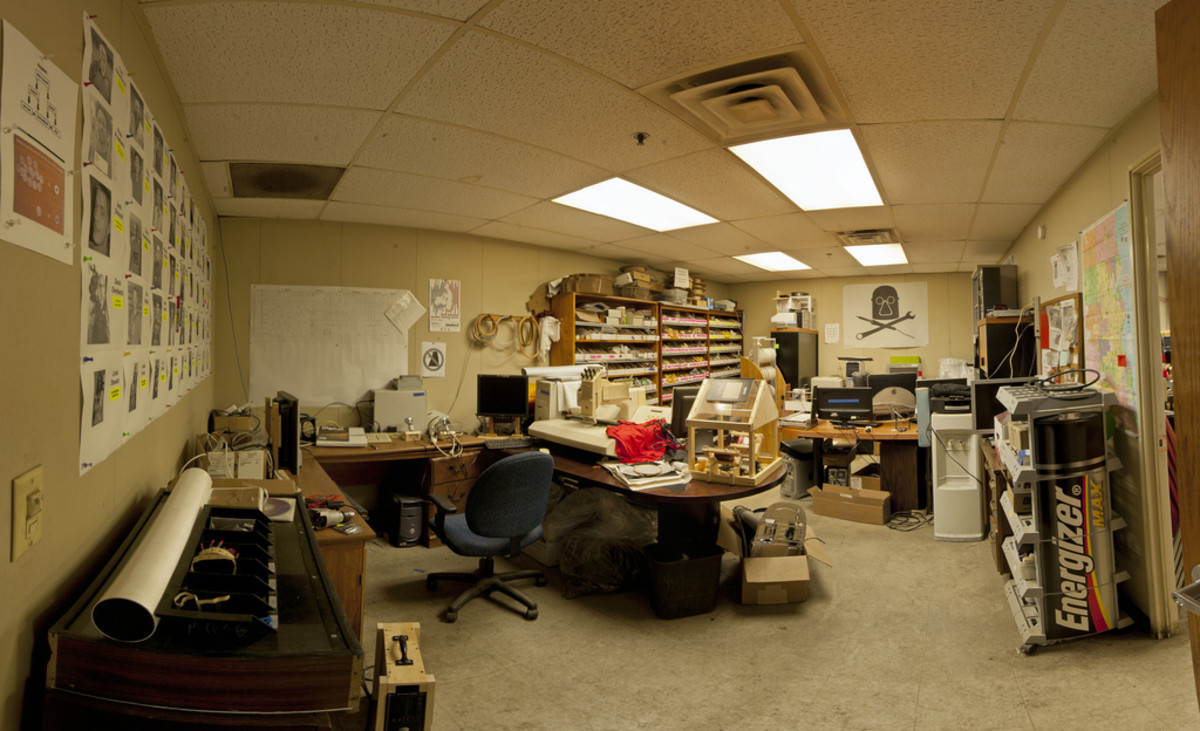
\includegraphics[width=\paperwidth]{milwaukee-makerspace.jpg}}
    \begin{frame}{\boxx{Milwaukee Makerspace}}
      \photoby{Pete Prodoehl}{https://secure.flickr.com/photos/raster/6799480743/}{CC by-nc-sa}
    \end{frame}
  }

  \begin{frame}{Menschen}
    \concept{Hacker}{
      In einem übergreifenden Sinn umfasst \textsl{Hacker}
      experimentierfreudige Personen, die mit ihren Fachkenntnissen eine
      Technologie beliebiger Art außerhalb ihrer normalen Zweckbestimmung oder
      ihres gewöhnlichen Gebrauchs benutzen. (Wikipedia)
    }
    \pause
    \textsl{Die Anwendbarkeit des generischen Maskulinum ist umstritten. Daher
    existiert der Begriff “Häckse” für eine weibliche Person und “Hackspace” als
    neutraler Begriff für den Raum.}
  \end{frame}

  {
    \pagecolor{black}
    \color{white}
    \usebackgroundtemplate{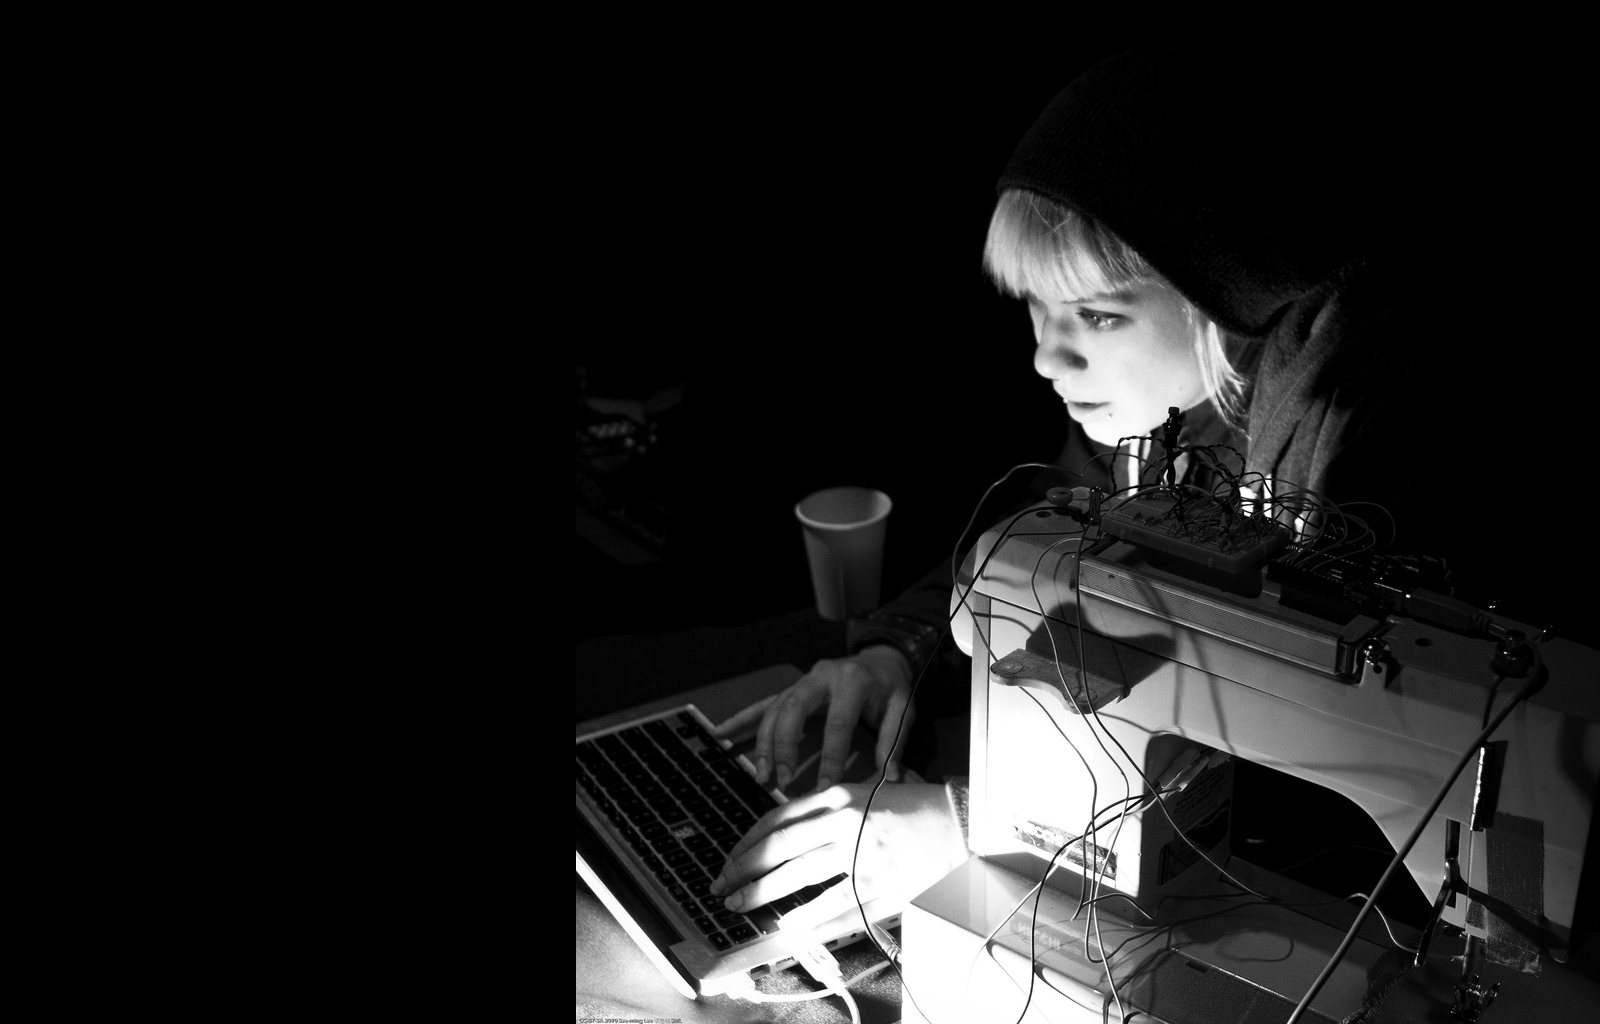
\includegraphics[width=\paperwidth]{hacker.jpg}}
    \begin{frame}{\boxx{Musizieren mit der Nähmaschine}}
      \photoby{See-Ming Lee}{https://secure.flickr.com/photos/seeminglee/4390053625/}{CC by-sa}
    \end{frame}
  }

  \begin{frame}{Aktivitäten}
    \begin{itemize}
      \item Do It Yourself
      \item Workshops
      \item Vorträge
      \item Teilen von Wissen
      \item Spaß haben
    \end{itemize}
  \end{frame}

  {
    \usebackgroundtemplate{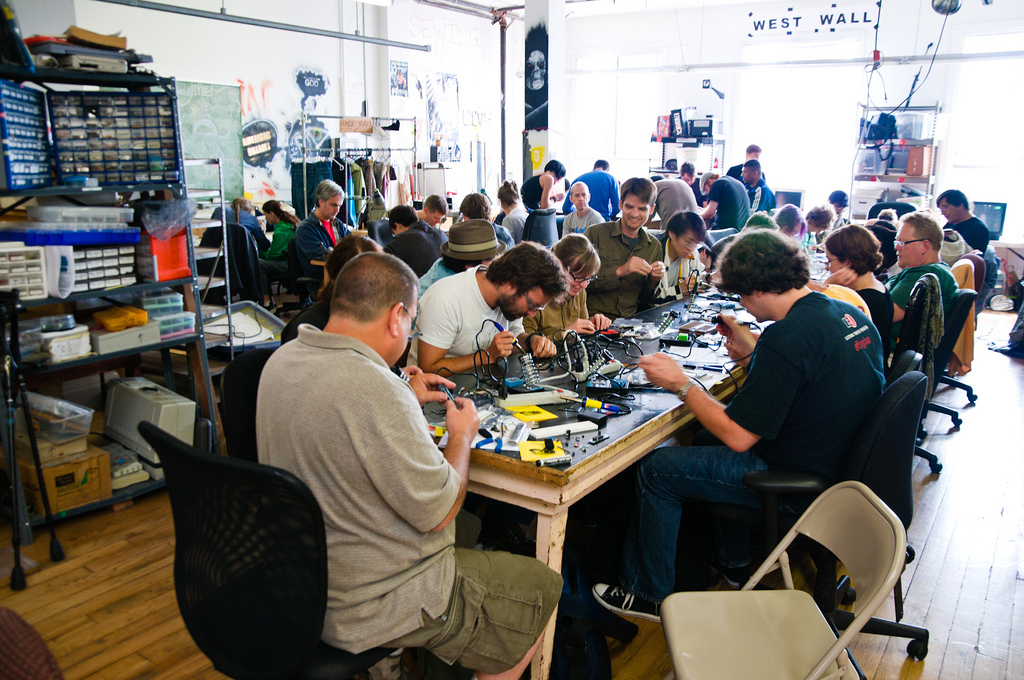
\includegraphics[width=\paperwidth]{workshop.jpg}}
    \begin{frame}{\boxx{Workshop}}
      \photoby{maltman23}{https://secure.flickr.com/photos/maltman23/5982427147/}{CC by-sa}
    \end{frame}
  }

  \begin{frame}{Infrastruktur}
    \begin{itemize}
      \item Strom
      \item Computer-Netzwerk
      \item Internetzugang
      \item Werkzeuge und Maschinen
      \item Getränke
    \end{itemize}
  \end{frame}

  {
    \usebackgroundtemplate{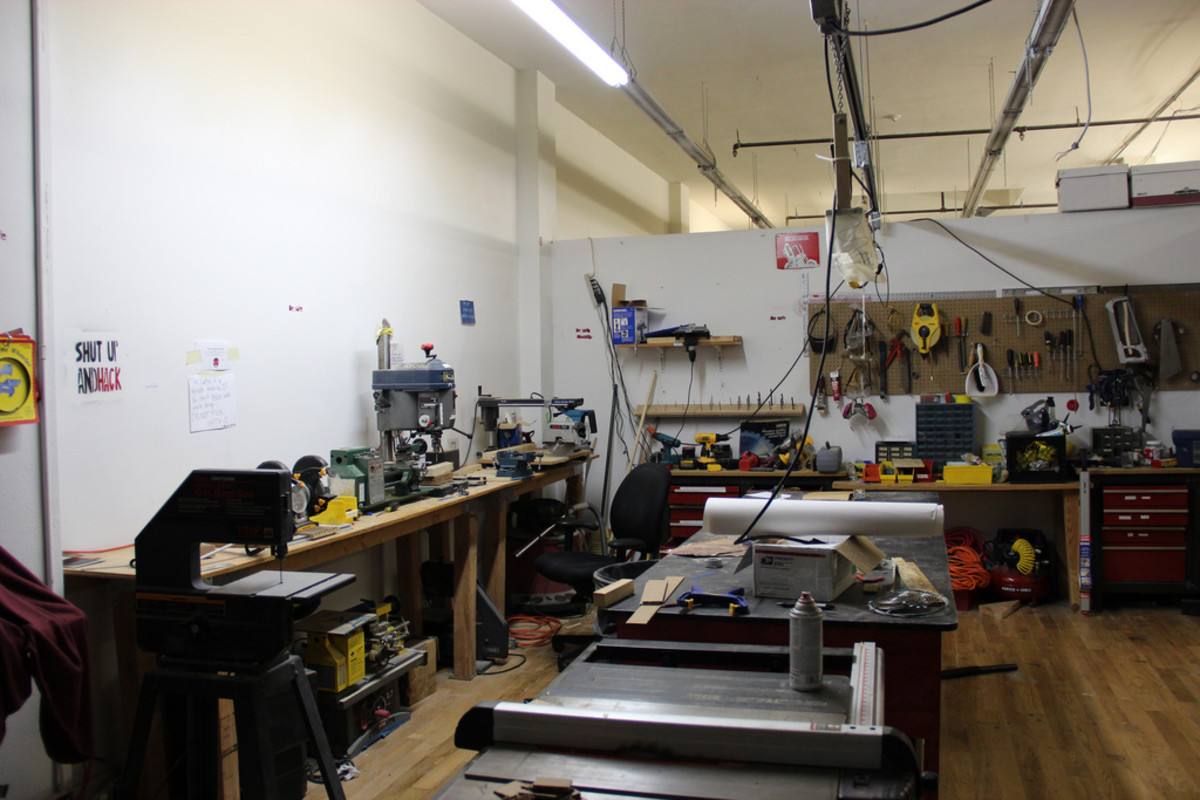
\includegraphics[width=\paperwidth]{infrastructure.jpg}}
    \begin{frame}{\boxx{Werkstatt}}
      \photoby{dreamexplorer}{https://secure.flickr.com/photos/dreamexplorer/5739464898/}{CC by-nc-sa}
    \end{frame}
  }

  \subsection{Bestehende Projekte}

  {
    \usebackgroundtemplate{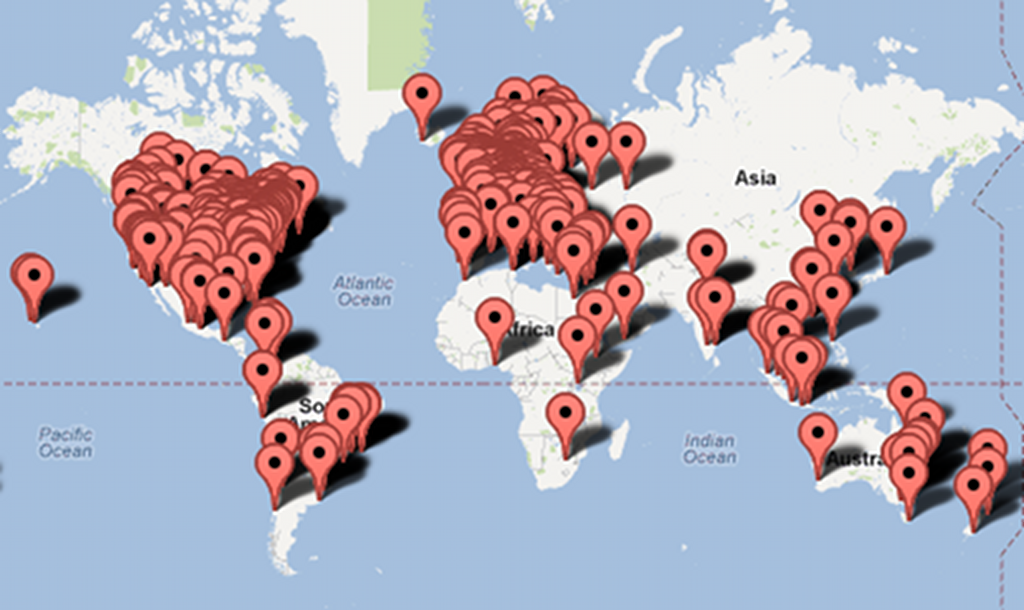
\includegraphics[width=\paperwidth]{hackerspaces-map.png}}
    \begin{frame}{\boxx{visit ALL the hackerspaces}}
      \photoby{hackerspaces.org}{http://hackerspaces.org/wiki/List\_of\_Hacker\_Spaces}{geklaut}
    \end{frame}
  }


  {
    \usebackgroundtemplate{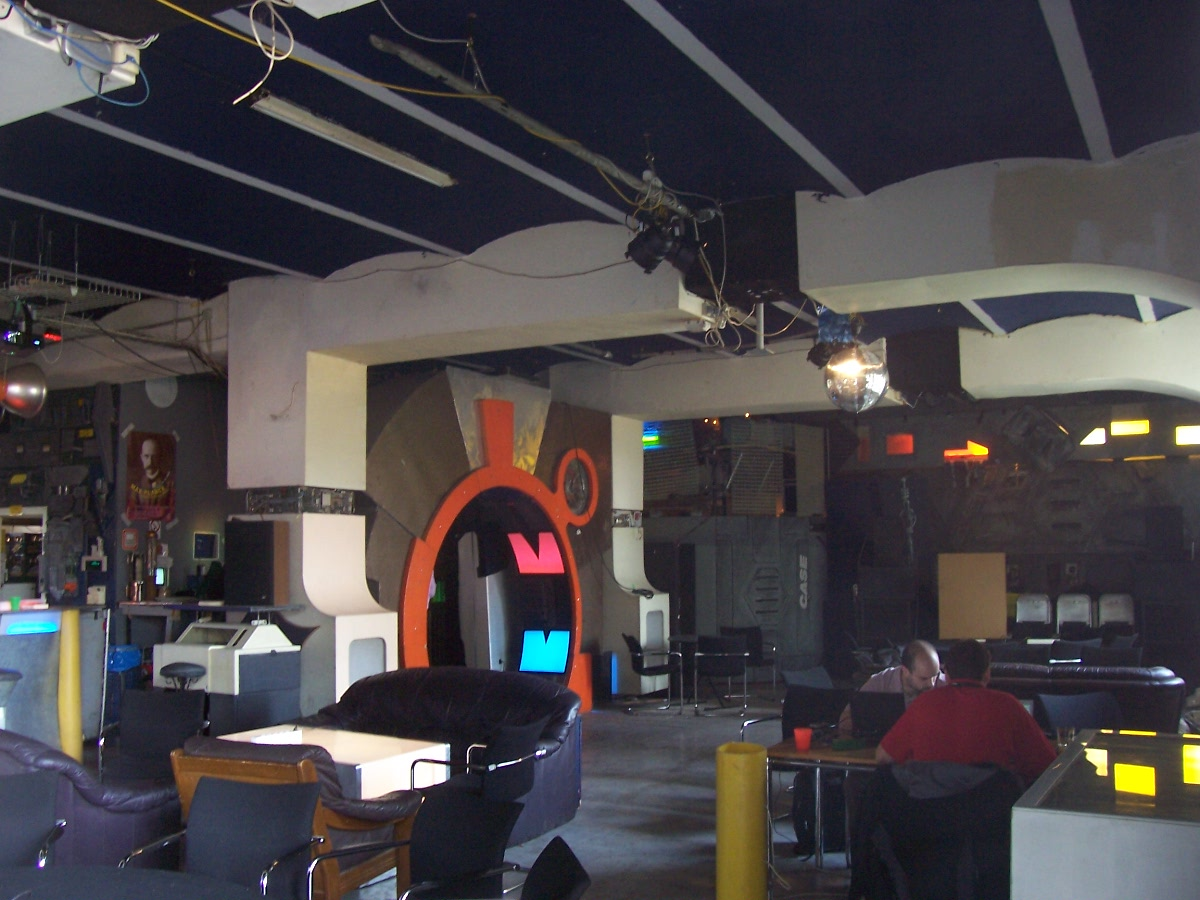
\includegraphics[width=\paperwidth]{c-base.jpg}}
    \begin{frame}{\boxx{c-base}}
      \photoby{Berto Garcia}{https://secure.flickr.com/photos/bertogg/2876753569/}{CC by-sa}
    \end{frame}
  }

  \begin{frame}
    \begin{columns}[l]
      \column{.5\textwidth}
      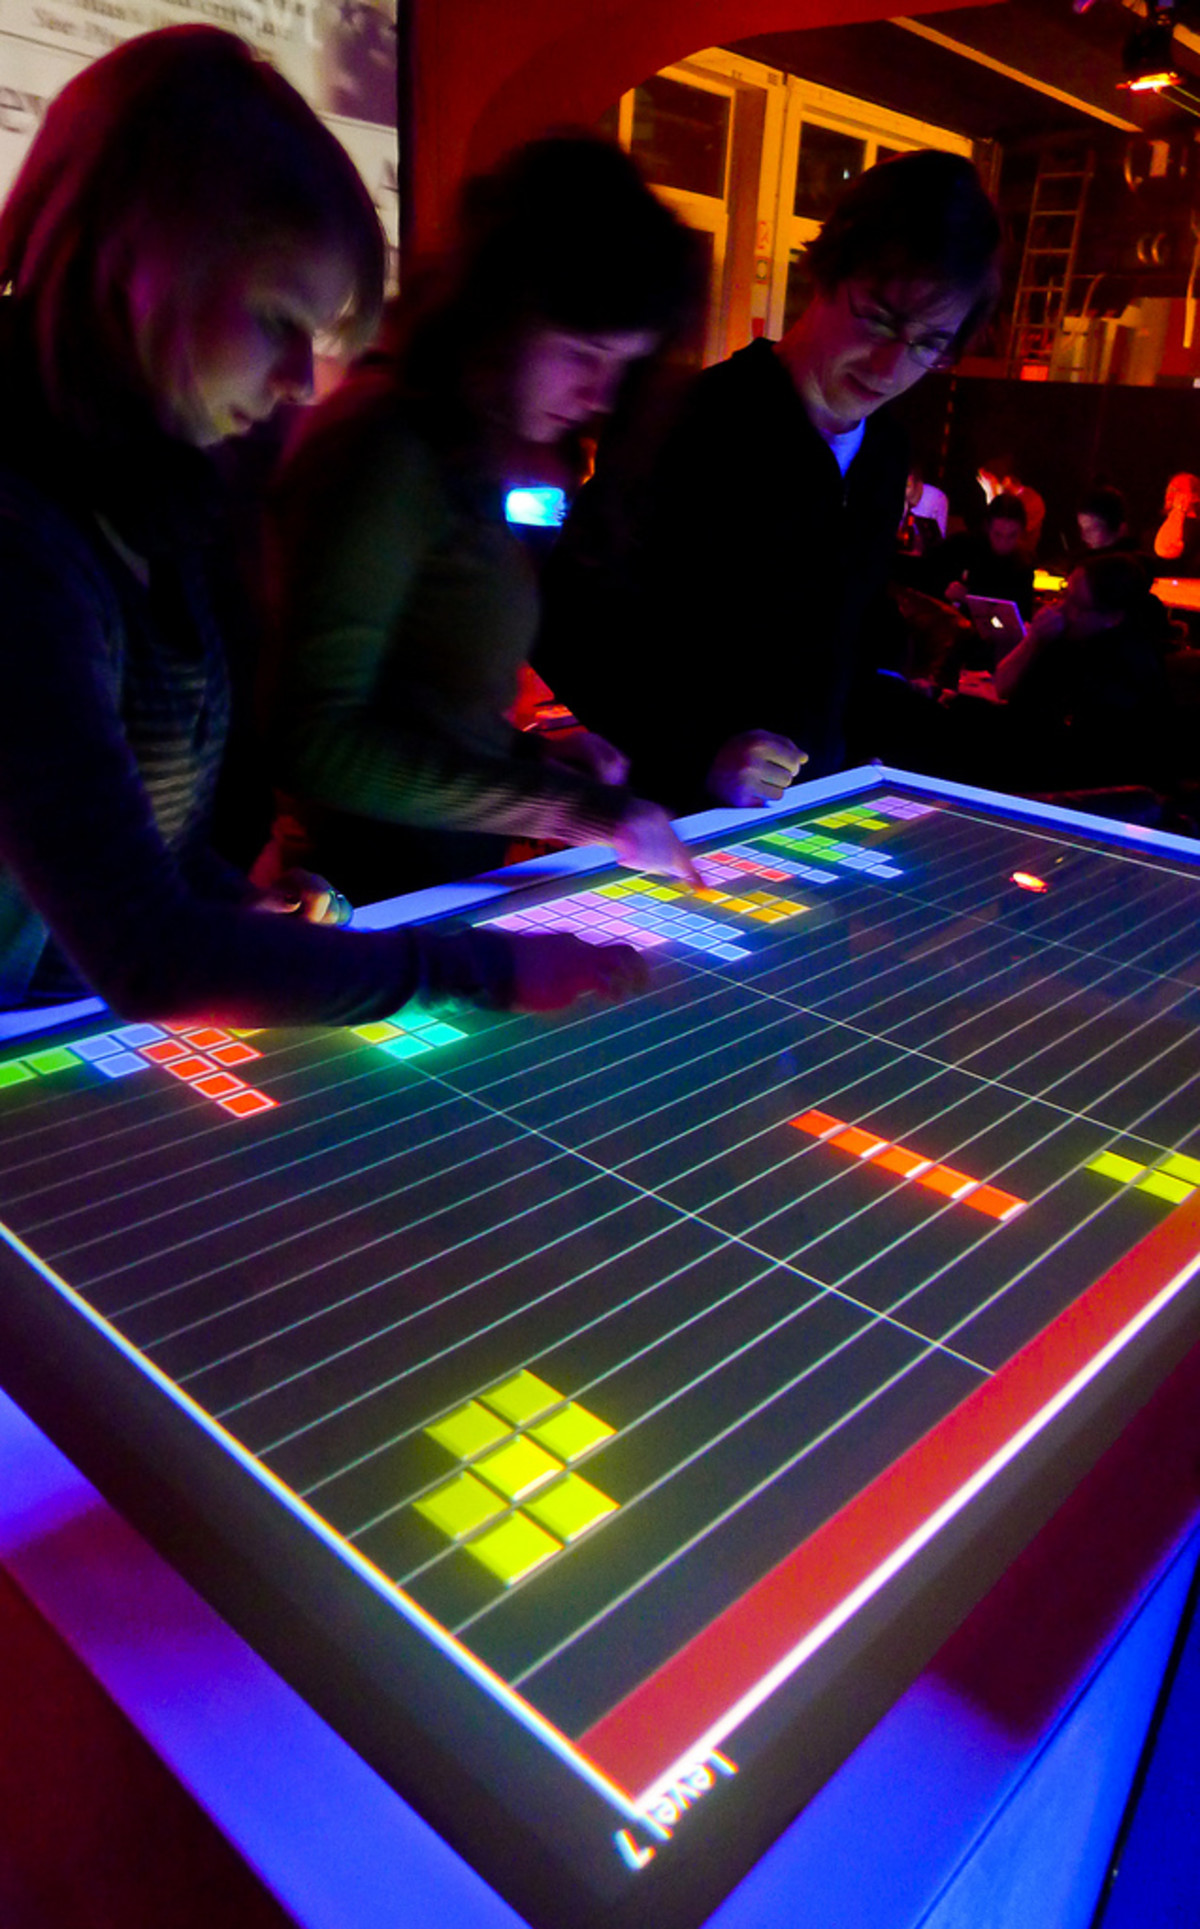
\includegraphics[width=0.8\textwidth]{multitouch-tetris.jpg}
      \column{.5\textwidth}
      c-base
      \begin{itemize}
        \item Gegründet 1995\\in Berlin
        \item ca. 723 $m^2$
        \item 350 Mitglieder
        \item Raumstation (abgestürzt)
        \item Veranstaltungsraum
        \item Seminarraum
        \item Werkstätten
      \end{itemize}
    \end{columns}
  \end{frame}


  {
    \usebackgroundtemplate{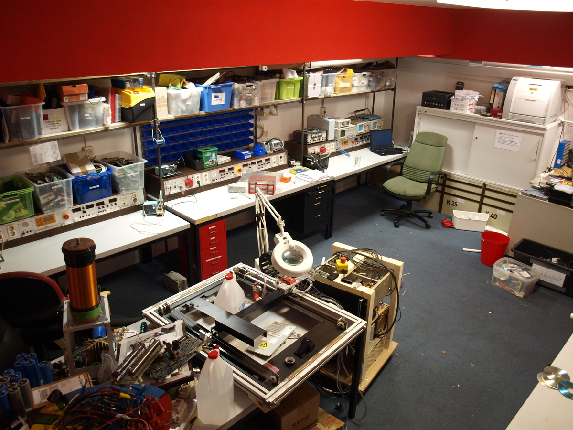
\includegraphics[width=\paperwidth]{daslabor.jpg}}
    \begin{frame}{\boxx{Das Labor}}
      \photoby{Das Labor}{http://das-labor.org/wiki/Datei:Bastelraum\_1.JPG}{GNU FDL}
    \end{frame}
  }

  \begin{frame}
    \begin{columns}[l]
      \column{.5\textwidth}
      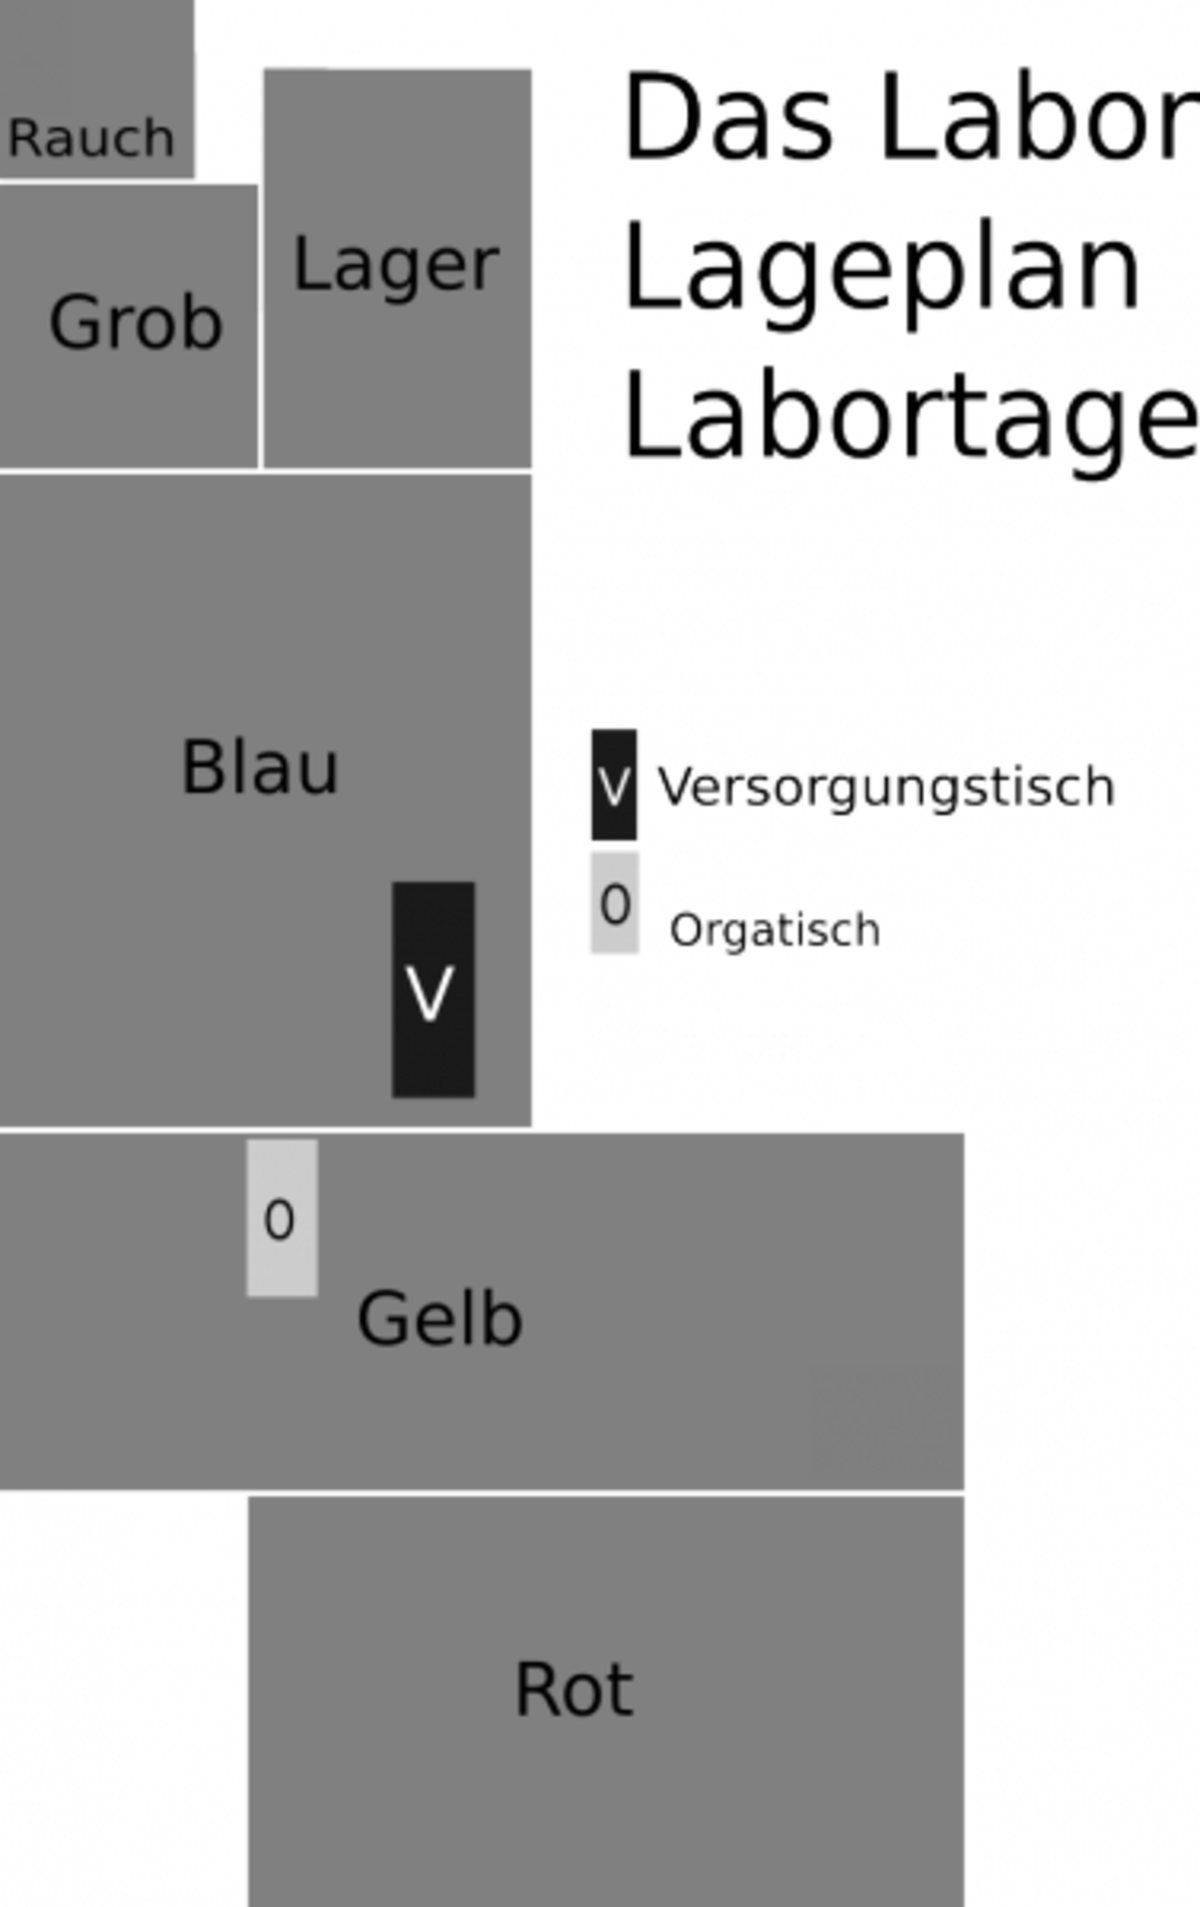
\includegraphics[width=0.8\textwidth]{daslabor-map.png}
      \column{.5\textwidth}
      Das Labor
      \begin{itemize}
        \item Gegründet 2007\\in Bochum
        \item ca. 180 $m^2$
        \item Seminarraum (Blau)
        \item Elektronik-Werkstatt (Rot)
        \item Metallwerkstatt (Grob)
        \item Küche (Blau)
        \item Wohnzimmer (Gelb)
        \item Raucherzimmer (Rauch)
      \end{itemize}
    \end{columns}
  \end{frame}

  {
    \usebackgroundtemplate{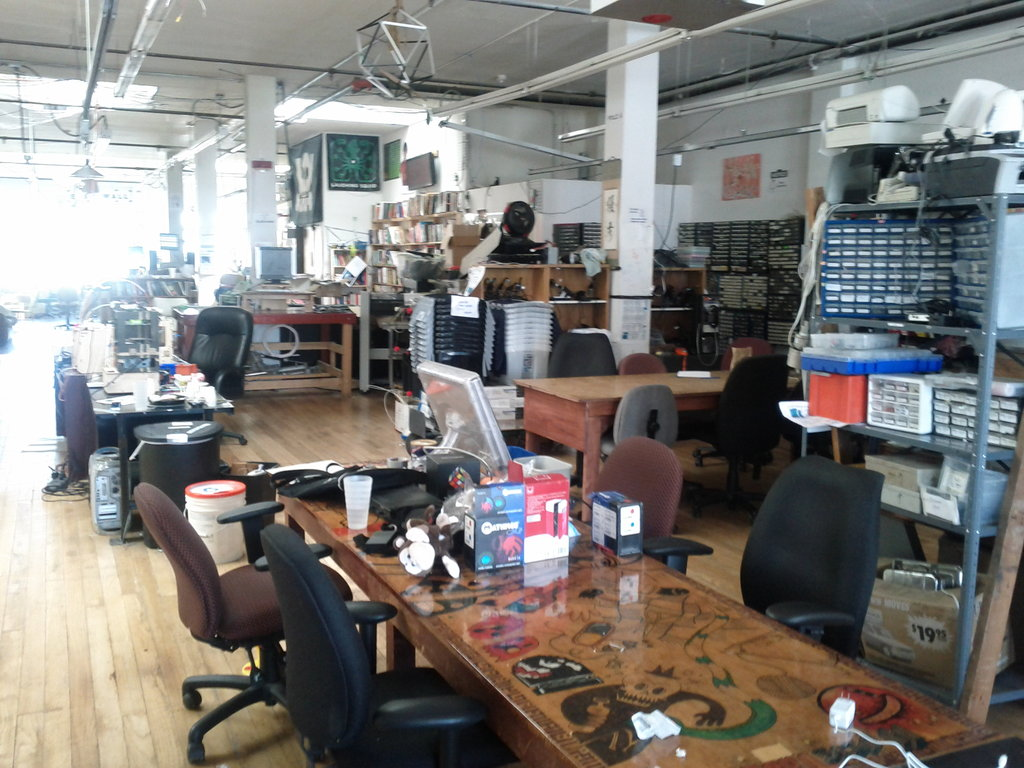
\includegraphics[width=\paperwidth]{noisebridge.jpg}}
    \begin{frame}{\boxx{Noisebridge}}
      \photoby{sd}{https://secure.flickr.com/photos/sd/5705133826/}{CC by-nc-sa}
    \end{frame}
  }

  \begin{frame}
    \begin{columns}[l]
      \column{.5\textwidth}
      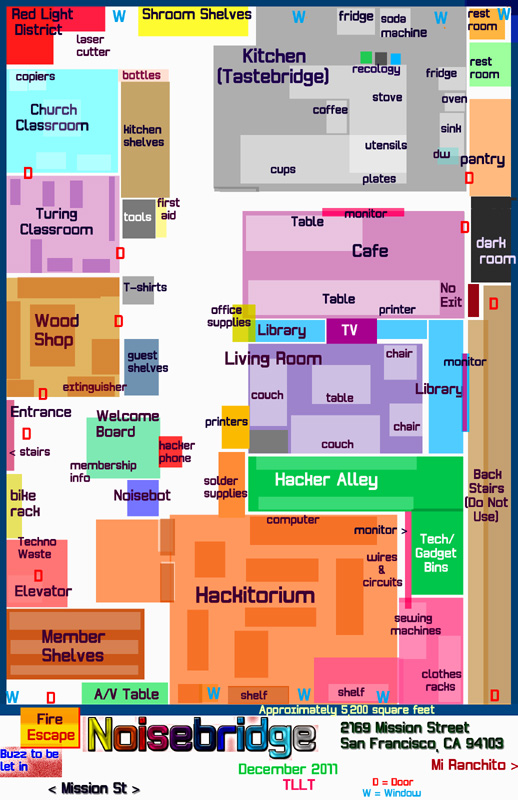
\includegraphics[width=0.8\textwidth]{noisebridge-map.jpg}
      \column{.5\textwidth}
      Noisebridge
      \begin{itemize}
        \item Gegründet 2007\\in San Francisco
        \item 483 $m^2$ Großraum
        \item 2 Seminarräume
        \item Hackcenter
        \item Laser-Labor
        \item Holzwerkstatt
        \item Schneiderrei
        \item Küche
        \item Café
        \item Wohnzimmer
      \end{itemize}
    \end{columns}
  \end{frame}


  \subsection{Muster und Antimuster}

  \begin{frame}{Design Pattern}
    \concept{Entwurfsmuster}{Bewährte Lösungsschablonen für bestimmte, wiederkehrende Probleme}
  \end{frame}

  \begin{frame}{Anti-Pattern}
    \concept{Antimuster}{Häufig anzutreffende schlechte Lösungsansatze für bestimmte Probleme}
  \end{frame}

  \section{Design Patterns}

  \subsection{Nachhaltigkeit}

  \begin{frame}{Infrastruktur}
    \pattern{
      Huhn oder Ei?\\
      Was sollte zuerst realisiert werden?\\
      Infrastruktur oder Projekte?
    }{
      Infrastructure first!\\
      Neue Leute werden kommen.
    }
  \end{frame}

  \begin{frame}{Grace Hopper}
    \pattern{
      Sollen wir den Hackspace jetzt wirklich aufmachen?\\
      Haben wir an alles gedacht?\\
      Woher wissen wir, ob wir startklar sind?
    }{
      \textbf{Ja klar!!!}
      \pause
      \begin{quote}
        Es ist einfacher\\
        hinterher um Vergebung zu bitten,\\
        als vorher um Erlaubnis.
      \end{quote}
      \pause
      Fange einfach an!
      Die Probleme wirst du auf dem Weg lösen.
    }
  \end{frame}

  {
    \usebackgroundtemplate{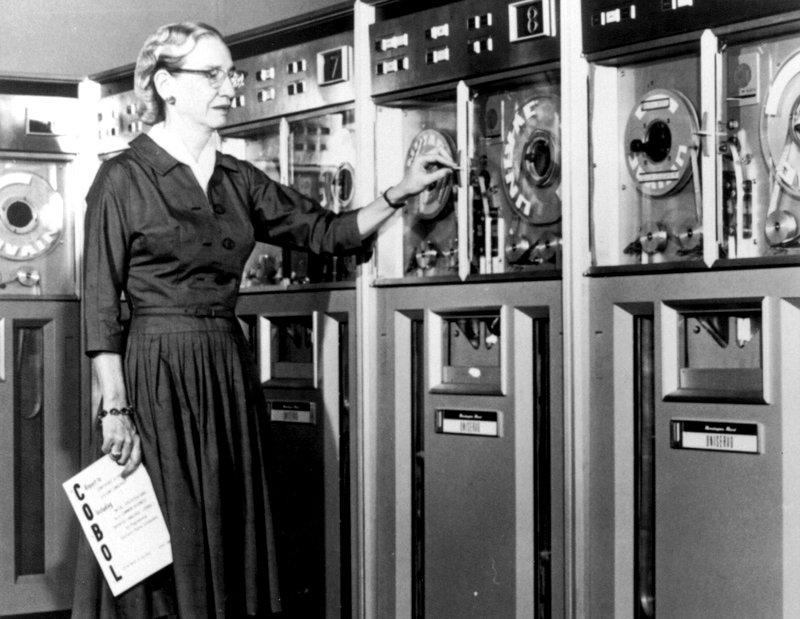
\includegraphics[width=\paperwidth]{grace-hopper.jpg}}
    \begin{frame}
      \large{
      \boxx{Grace Hopper}\\
      }
      \small{
      \boxx{Entwarf einen der ersten Compiler}\\
      \boxx{Hat die Programmiersprace COBOL entwickelt}\\
      \boxx{Prägte den Begriff \textsl{Debugging}}\\
      }
      \photoby{miss karen}{https://secure.flickr.com/photos/misbehave/2782902040/}{CC by}
    \end{frame}
  }



  \begin{frame}{Kollektiv}
    \pattern{
      Wie sollte die Gruppe kommunizieren?\\
      Beim Stammtisch? Per Telefon?
    }{
      Was tut ein echter Hacker*?\\
      \pause
      \begin{enumerate}
        \item{IRC oder Jabber für Sofortnachrichten}
        \pause
        \item{Mailingliste für Diskussionen}
        \pause
        \item{Wiki für Dokumentation}
      \end{enumerate}
    }
  \end{frame}


  \begin{frame}{Kritische Masse}
    \pattern{
      Du willst als einzige* in deiner Stadt einen Hackspace eröffnen.\\
      Das wird nichts.
    }{
      \begin{itemize}
        \item{Daumenregel: $2+2$}
        \pause
        \item{Du brauchst einen Partner*}
        \pause
        \item{Zwei Leute mehr zum Loslegen}
        \pause
        \item{Zehn Leute machen einen guten Anfang}
      \end{itemize}
    }
  \end{frame}

  \begin{frame}{Starke Persönlichkeiten}
    \pattern{
      Nichts wird fertig.\\
      Alle wollen den Hackspace, aber ihr tut euch schwer, den Hintern hochzukriegen.
    }{
      \begin{itemize}
        \item{Suche starke Persönlichkeiten}
        \pause
        \item{Experience != Commitment}
        \pause
        \item{Autorität besitzen und nicht ausnutzen}
      \end{itemize}
    }
  \end{frame}

  \subsection{Unabhängigkeit}

  \begin{frame}{Hausbesitzer und Nachbarschaft}
    \pattern{
      Du hast den perfekten Raum gefunden, aber der Hausbesitzer scheint
      merkwürdig zu sein. Außerdem sind die Nachbarn meckrig.
    }{
      \begin{itemize}
        \item{Hausbesitzer neutral und großzügig?}
        \pause
        \item{Nachbarn cool und kommunikativ?}
        \pause
        \item{Hacker* leben nicht wie die Mehrheit}
      \end{itemize}
    }
  \end{frame}

  \begin{frame}{Anti-Mitbewohner}
    \pattern{
      Ihr braucht viel Platz für Treffen, Werkstatt, Lagerraum und
      Arbeitsflächen für Materialien und Projekte. Um die Miete zu senken oder
      aus sympathie denkt ihr, dass es großartig wäre, wenn ein Mensch in eurem
      Space lebt. Aber irgendwie klappt das nicht, weil du die Werkstatt nicht
      mehr nutzen kannst.
    }{
      \begin{itemize}
        \item{Übernachten ist voll okay}
        \pause
        \item{Wohnen geht gar nicht}
        \pause
        \item{Schmeißt Mitbewohner notfalls raus}
      \end{itemize}
    }
  \end{frame}

  \begin{frame}{Séparée}
    \pattern{
      Ihr wollt chillen, diskutieren oder in Kleingruppen arbeiten. Aber der
      Hauptraum ist voll besetzt: es sind einfach zu viele Leute im Space. Oder
      ihr wollt eine Zigarette rauchen, ohne die anderen zu stören.
    }{
      \begin{itemize}
        \item{Kleine separate Räume suchen/bauen}
        \pause
        \item{Trennung zwischen Hauptraum und Rest}
        \pause
        \item{Rauchen nur in deklarierten Räumen}
      \end{itemize}
    }
  \end{frame}

  \begin{frame}{Küche}
    \pattern{
      Als menschliches Wesen benötigst du Nahrung.\\
      Als Hacker* benötigst du Koffein und Nahrung zu ungewöhnlichen Uhrzeiten.
    }{
      \begin{itemize}
        \item{Richtet eine Küche ein!}
        \pause
        \item{Gemeinsames Kochen verbindet.}
        \pause
        \item{Spülmaschine}
        \pause
        \item{Kochen beibringen}
      \end{itemize}
    }
  \end{frame}

  {
    \usebackgroundtemplate{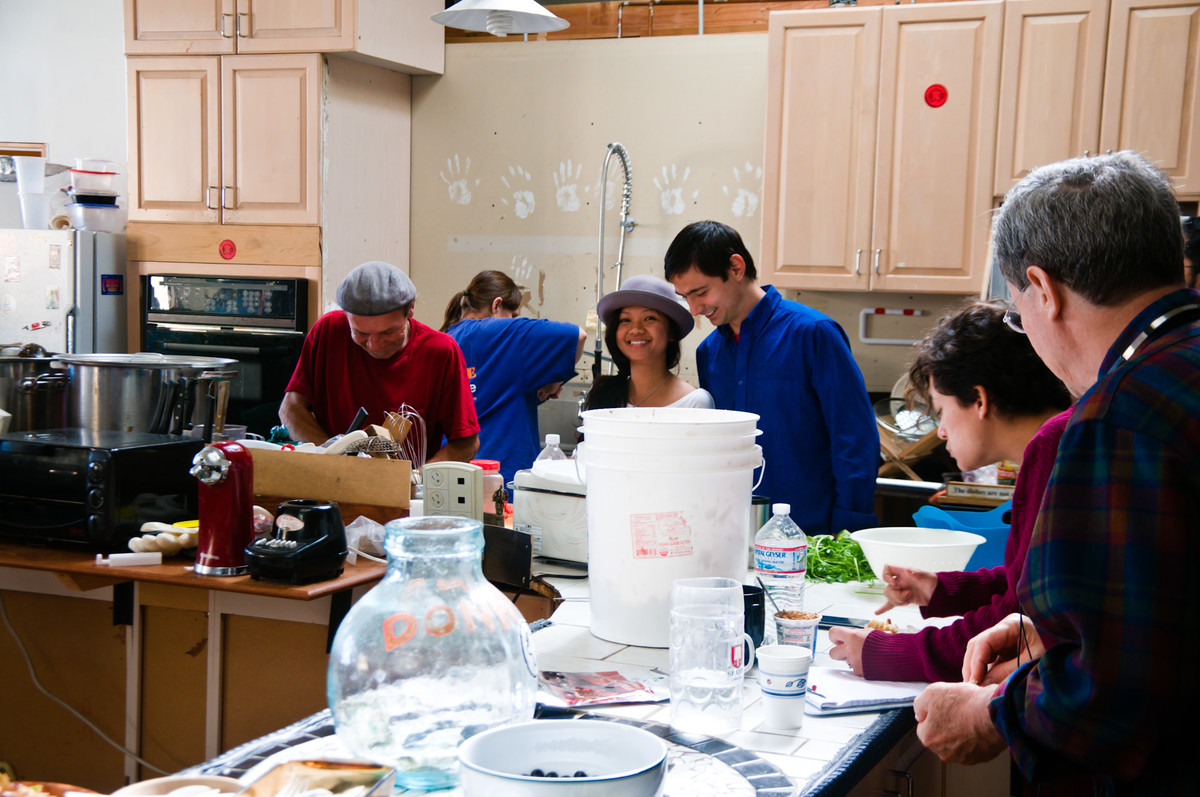
\includegraphics[width=\paperwidth]{kitchen.jpg}}
    \begin{frame}{\boxx{Küche der Noisebridge}}

      \photoby{maltman23}{https://secure.flickr.com/photos/maltman23/6254785979/}{CC by-sa}
    \end{frame}
  }

  \begin{frame}{Behaglichkeit}
    \pattern{
      All work and no play makes Jack a dull boy.\\
      Da muss noch was anderes sein, als Arbeitsplätze und Elektronikkrempel.
    }{
      \begin{itemize}
        \item{Sofas, bequeme Stühle, Tische, Aschenbecher, stimmungsvolle Beleuchtung, ein Soundsystem, Beamer und Videospiele}
        \pause
        \item{Pflanzen?}
      \end{itemize}
    }
  \end{frame}

  {
    \usebackgroundtemplate{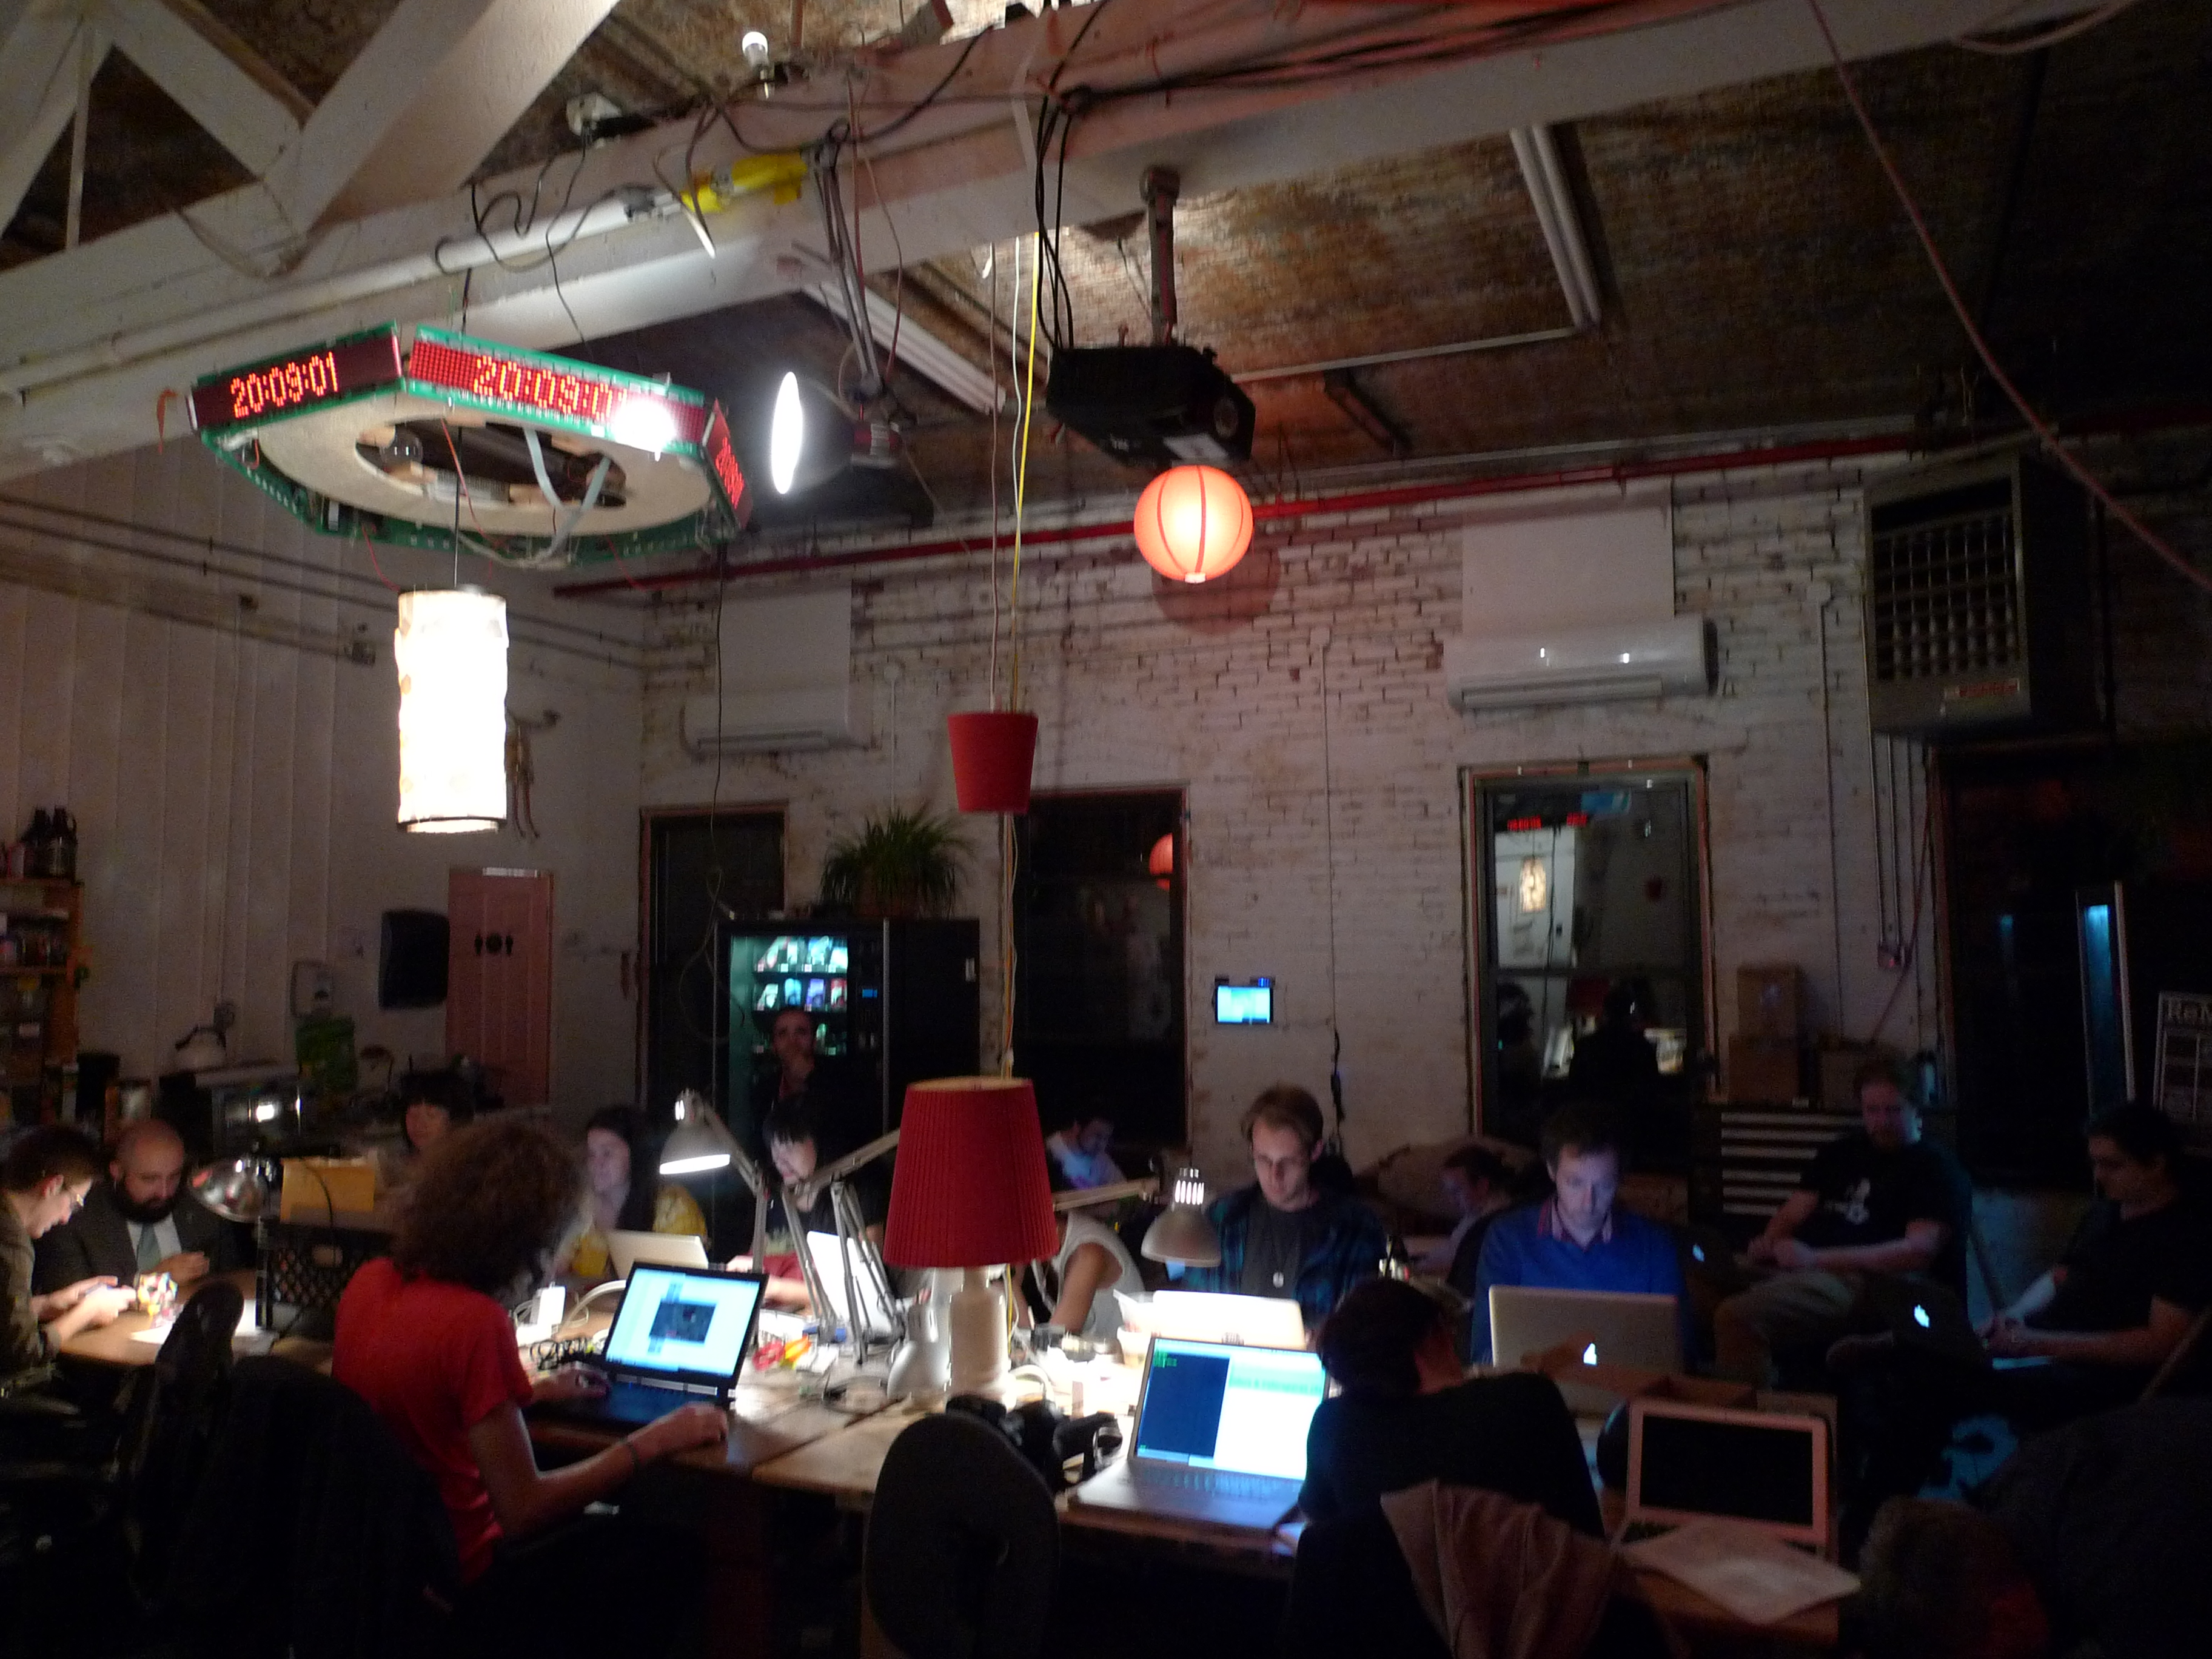
\includegraphics[width=\paperwidth]{coziness.jpg}}
    \begin{frame}{\boxx{Beleuchtung im NYC Resistor}}
      \photoby{girl\_onthe\_les}{https://secure.flickr.com/photos/girlontheles/6164704739/}{CC by-nc-nd}
    \end{frame}
  }

  \begin{frame}{Dusche}
    \pattern{
      Nach langen Hacking Sessions werdet ihr anfangen, komisch zu riechen.\\
      Außerdem scheinen die Gäste in eurem Space Körperpflege zu
      vernachlässigen.
    }{
      \begin{itemize}
        \item{Badezimmer mit Dusche einrichten}
        \pause
        \item{Duschen entspannt und inspiriert}
        \pause
        \item{Gäste können tagelang bleiben}
        \pause
        \item{Waschmaschine}
      \end{itemize}
    }
  \end{frame}

  \begin{frame}{Mitgliedsbeiträge}
    \pattern{
      Ihr braucht Geld für die Miete und Ausrüstung.\\
      Größere Projekte brauchen Unterstützung.
    }{
      \begin{itemize}
        \item{Sammelt regelmäßig Beiträge ein!}
        \pause
        \item{Macht niemals Ausnahmen}
        \pause
        \item{Angemessener Beitrag mit Ermäßigung nach Selbsteinschätzung}
        \pause
        \item{3 Monate Miete auf dem Konto halten}
        \pause
        \item{Pedantischen Kassenwart* wählen}
      \end{itemize}
    }
  \end{frame}

  \begin{frame}{Anti-Sponsoring}
    \pattern{
      Ihr glaubt, dass es eine gute Idee ist, bei einer wohlgesonnenen Firma
      unterzukommen. Oder in einer Universität, weil die meisten von euch
      ohnehin Studis sind.
    }{
      \begin{itemize}
        \item{Niemals von externen Sponsoren abhängig machen}
        \pause
        \item{Spenden annehmen, aber nicht darauf verlassen}
        \pause
        \item{Auch nette Firmen unterliegen Zwängen (Kapitalismus)}
      \end{itemize}
    }
  \end{frame}

  \subsection{Regelmäßigkeit}

  \begin{frame}{Plenum}
    \pattern{
      Ihr wollt interne Konflikte lösen, demokratische Entscheidungsfindung
      ausüben, laufende Probleme und Pläne für die Zukunft besprechen.
    }{
      \begin{itemize}
        \item{Regelmäßig mit allen Mitgliedern treffen}
        \pause
        \item{Tagesordnung vorbereiten und Ziele setzen}
        \pause
        \item{Verantwortung übergeben}
        \pause
        \item{Protokoll schreiben und verteilen}
        \pause
        \item{Ein Mal pro Woche}
      \end{itemize}
    }
  \end{frame}

  {
    \usebackgroundtemplate{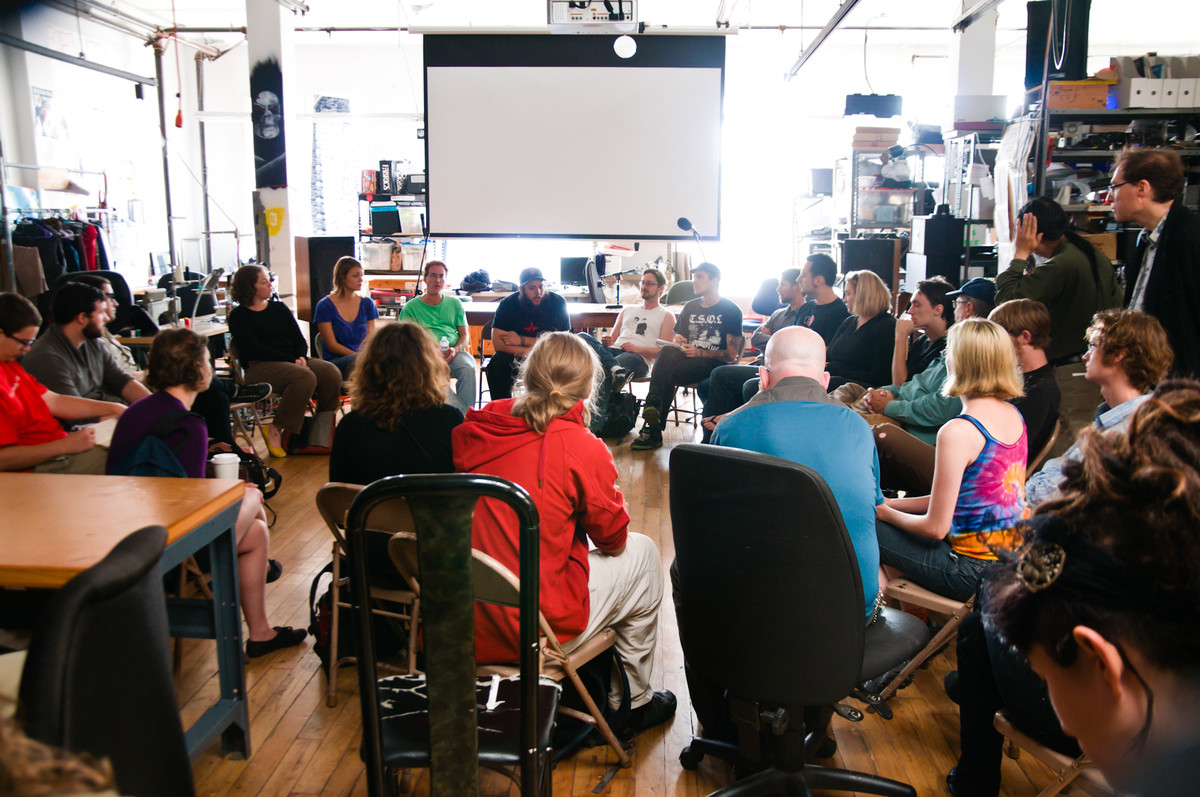
\includegraphics[width=\paperwidth]{meetup.jpg}}
    \begin{frame}{\boxx{Treffen in der Noisebridge}}
      \photoby{maltman23}{https://secure.flickr.com/photos/maltman23/6255313258/}{cc-by-sa}
    \end{frame}
  }

  \begin{frame}{Dienstag}
    \pattern{
      Jeder Wochentag ist ungünstig. Ihr findet keinen Tag, an dem alle Zeit
      haben. Irgendwer hat immer einen anderen Termin.
    }{
      \begin{itemize}
        \item{Dienstag. Ende der Diskussion.}
      \end{itemize}
    }
  \end{frame}

  \begin{frame}{OpenChaos}
    \pattern{
      Ihr wollt neue Leute anziehen und eine Verbindung zur äußeren Welt herstellen.
    }{
      \begin{itemize}
        \item{Monatlicher Vortrag oder Workshop}
        \pause
        \item{Ordentlich ankündigen (Ortszeit, Alter!)}
        \pause
        \item{Interessierte einladen, Spinnern verschweigen}
      \end{itemize}
    }
  \end{frame}

  {
    \usebackgroundtemplate{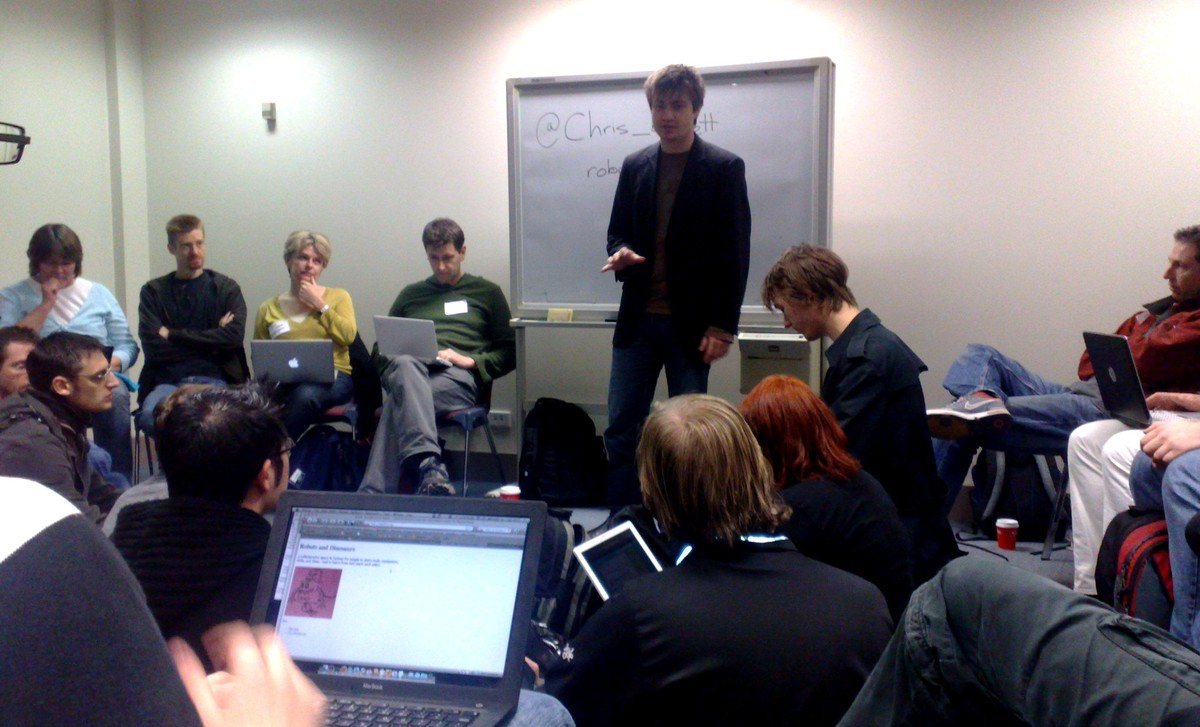
\includegraphics[width=\paperwidth]{talk.jpg}}
    \begin{frame}{\boxx{Vortrag im Robots and Dinosaurs}}
      \photoby{Alegrya}{https://secure.flickr.com/photos/alegrya/3670712239/}{CC by-nc-sa}
    \end{frame}
  }


  \begin{frame}{U23}
    \pattern{
      Ältere Mitglieder machen ihren Abschluss oder heiraten.\\
      Euer Space braucht junges Blut.
    }{
      \begin{itemize}
        \item{Wettbewerbe organisieren}
        \pause
        \item{Miteinander statt Gegeneinander}
        \pause
        \item{Anleiten und Raum zu Experimentieren geben}
        \pause
        \item{Kluge Leute für den Hackspace rekrutieren}
      \end{itemize}
    }
  \end{frame}

  \begin{frame}{Sinuskurve}
    \pattern{
      Ihr habt alles richtig gemacht. Ein paar schöne Events und eine tolle
      Zeit in eurem flauschigen Hackspace liegen zurück. Nach einiger Zeit
      jedoch geht der Enthusiasmus zurück und die Projekte stagnieren.
    }{
      \begin{itemize}
        \item{Enthusiasmus sinusförmig}
        \pause
        \item{Zyklus: vier Jahre}
        \pause
        \item{Durchhalten}
      \end{itemize}
    }
  \end{frame}

  \subsection{Konfliktlösung}

  \begin{frame}{Konsens}
    \pattern{
      Ihr müsst eine Entscheidung treffen, die die ganze Gruppe betrifft und
      wollt sicherstellen, dass niemand übergangen wird.
    }{
      \begin{itemize}
        \item{Nicht abstimmen}
        \pause
        \item{Lösungsorientiert diskutieren}
        \pause
        \item{Beschließen, wenn alle einverstanden sind}
      \end{itemize}
    }
  \end{frame}

  \begin{frame}{Demokratie}
    \pattern{
      Ihr müsst eine Entscheidung treffen, die die ganze Gruppe betrifft.\\
      Aber die Diskussion scheint nicht zu einer Einigung zu führen.
    }{
      \begin{itemize}
        \item{Wenn ihr es so wollt: Stimmt ab!}
        \pause
        \item{Stärkste Minderheit dominiert}
        \pause
        \item{Es wird sich zeigen}
      \end{itemize}
    }
  \end{frame}

  \begin{frame}{Befehl}
    \pattern{
      Niemand spült das Geschirr. Der Hackspace sieht hulle aus.\\
      Keinen scheint das zu kümmern.
    }{
      \begin{itemize}
        \item{Befehle Leute zum Arbeiten}
        \pause
        \item{Beschwere dich, schreie rum wenn nötig}
        \pause
        \item{Aber mache immer mit}
      \end{itemize}
    }
  \end{frame}

  \begin{frame}{sudo}
    \pattern{
      Ihr habt als eine Gemeinschaft gleichgesinnter losgelegt,\\
      jedoch ist da draus plötzlich eine Diktatur eines einzelnen Hackers* geworden.
    }{
      \begin{itemize}
        \item{Keine Ränge vergeben}
        \pause
        \item{Diktatur temporär nutzen}
        \pause
        \item{Root deaktivieren, sudo ins Logbuch}
      \end{itemize}
    }
  \end{frame}

  \begin{frame}{Verantwortung}
    \pattern{
      Du hast dich freiwillig gemeldet, um eine bestimmte, kritische Komponente
      eurer Infrastruktur zu verantworten (z.B. den Mailserver). Jedoch hast du
      auf einmal das Bedürfnis rumzuhängen.
    }{
      \begin{itemize}
        \item{Sei verantwortlich und stolz}
        \pause
        \item{Höre zu und bitte um Mithilfe}
        \pause
        \item{Übergebe den Job am Ende}
      \end{itemize}
    }
  \end{frame}

  \begin{frame}{Diskussionskultur}
    \pattern{
      Ihr seid mitten in eurem wöchentlichen Plenum.\\
      Alle schreien und nichts wird beschlossen.
    }{
      \begin{itemize}
        \item{Diskussionsfähigkeit muss gelernt werden}
        \pause
        \item{Leitung mit Sozialkompetenz}
        \pause
        \item{Nicht unterbrechen}
      \end{itemize}
    }
  \end{frame}

  \begin{frame}{Anti-Fahrradschuppen}
    \pattern{
      Du schlägst eine neue Einrichtung für euren Hackspace vor, wie z.B.
      einen Fahrradschuppen. Nun diskutieren alle über die Farbe. Und kein
      Fahrradschuppen wird gebaut.
    }{
      \begin{itemize}
        \item{Wer macht, hat Recht}
        \pause
        \item{Unnötige Komplexität vermeiden}
        \pause
        \item{Unnötige Diskussionen erkennen und beenden}
      \end{itemize}
    }
  \end{frame}

  {
    \usebackgroundtemplate{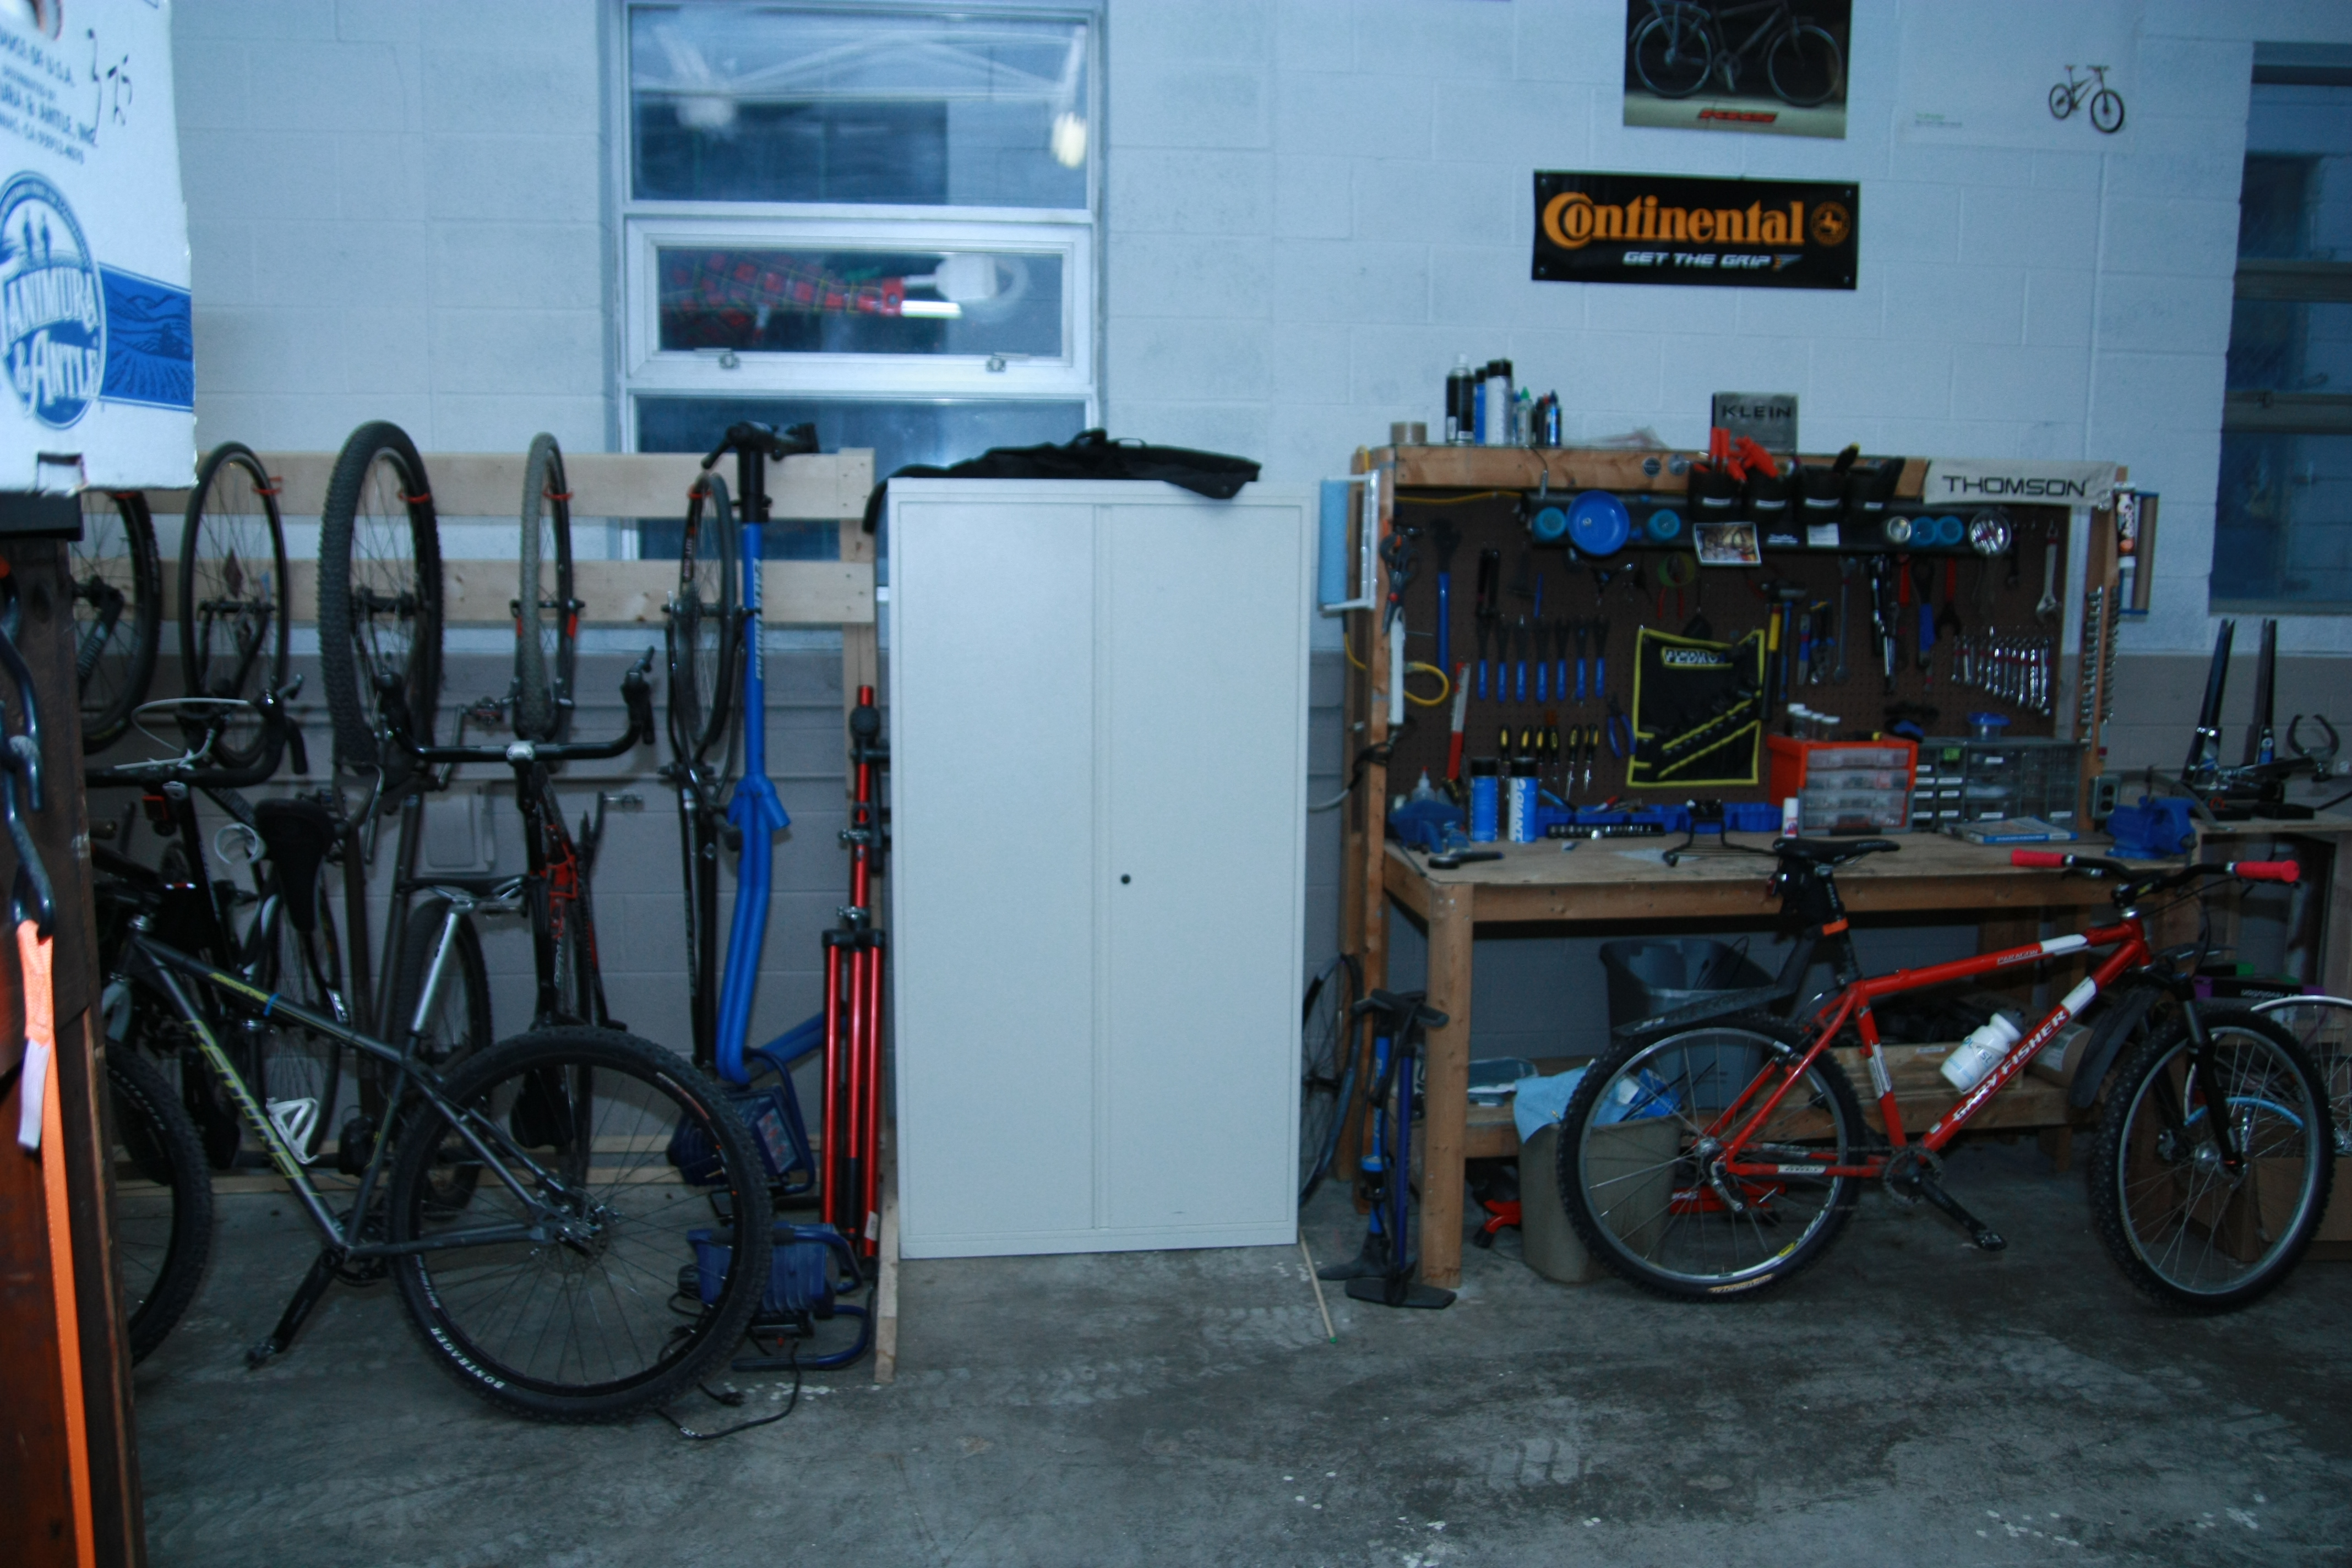
\includegraphics[width=\paperwidth]{bike-rack.jpg}}
    \begin{frame}{\boxx{Fahrradwerkstatt im i3 Detroit}}
      \photoby{Bradmcmahon}{https://secure.flickr.com/photos/bradmcmahon/5388909742/}{CC by-nc}
    \end{frame}
  }

  \begin{frame}{Privatgespräch}
    \pattern{
      Jemand löst ein Problem aus, das nicht in der Gruppe bewältigt werden kann.
    }{
      \begin{itemize}
        \item{Erfahrene Person spricht mit Störer*}
        \pause
        \item{Gut zuhören und Empfindung der Gruppe mitteilen}
        \pause
        \item{Störer* nicht exponieren}
      \end{itemize}
    }
  \end{frame}

  \subsection{Kreatives Chaos}

  \begin{frame}{Alte Hardware}
    \pattern{
      Du willst geile neue Hardware anschleppen, aber es ist keine Ecke mehr
      frei.\\Dein Hackspace ist ein Museum voller Müll geworden.
    }{
      \begin{itemize}
        \item{Alte Dinge auf Haufen sammeln}
        \pause
        \item{If you can hack it, you can have it!}
        \pause
        \item{In drei Stufen eskalieren und wegwerfen}
      \end{itemize}
    }
  \end{frame}

  \begin{frame}{Schlüssel zum Raum}
    \pattern{
      Du willst, dass der Space jederzeit zugänglich ist. Es ist keine Option,
      jemanden mitten in der Nacht anzurufen, nur um den Laden dicht zu machen,
      weil du nach Hause willst.
    }{
      \begin{itemize}
        \item{Schlüssel aushändigen und notieren}
        \pause
        \item{Sicheres Schloss, markierte Schlüssel}
        \pause
        \item{Pfand verlangen}
        \pause
        \item{Elektronisches Schließsystem macht “Spaß”}
      \end{itemize}
    }
  \end{frame}

  \begin{frame}{Club-Mate}
    \pattern{
      Ihr müsst Spenden sammeln. Ihr wollt nachts lange aufbleiben.\\Und ihr
      wollt einen richtig guten Eindruck machen – ohne Drogenkonsum.
    }{
      \begin{itemize}
        \item{Kauft eine Palette Club-Mate}
        \pause
        \item{Gegen feste Spende rausgeben}
      \end{itemize}
    }
  \end{frame}

  {
    \usebackgroundtemplate{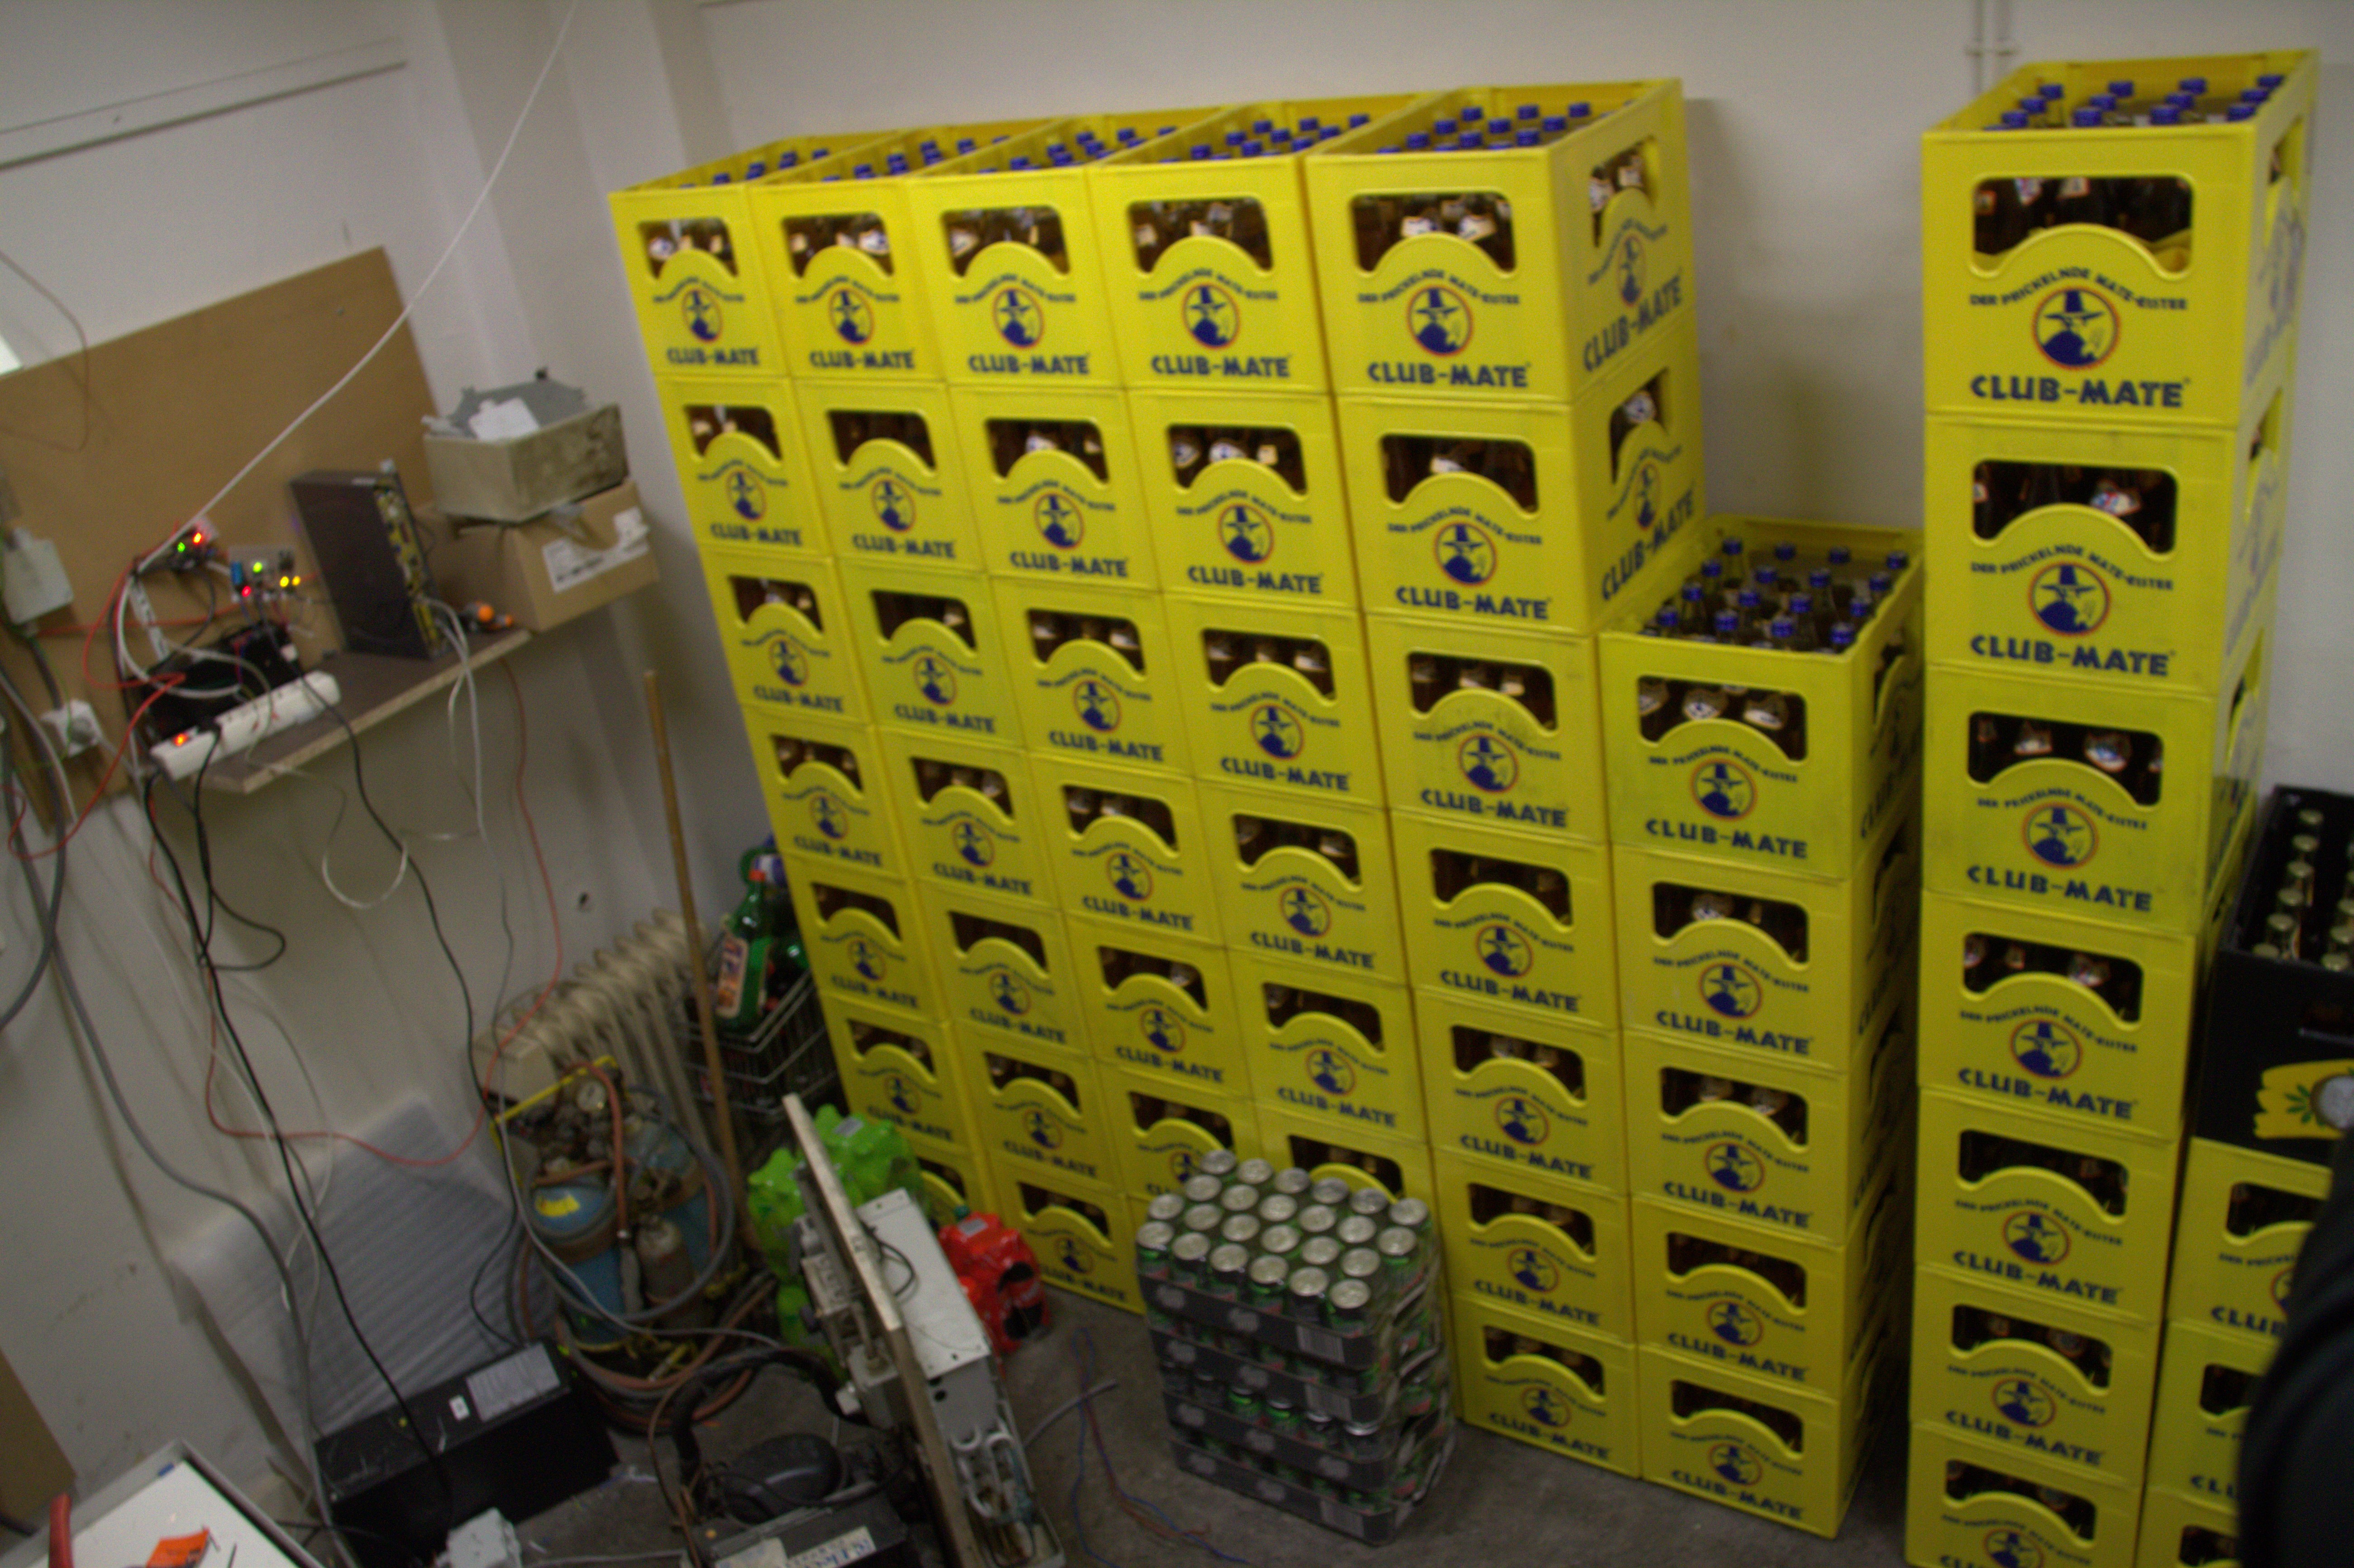
\includegraphics[width=\paperwidth]{club-mate.jpg}}
    \begin{frame}{\boxx{Club-Mate im Hack42}}
      \photoby{dvanzuijlekom}{https://secure.flickr.com/photos/dvanzuijlekom/6854225951/}{CC by-sa}
    \end{frame}
  }

  \section{Ausblick}

  \begin{frame}{Legt los!}
    \begin{itemize}
      \item Dies ist kein Kochbuch
      \pause
      \item Design Patterns entstehen aus Erfahrung
      \pause
      \item Findet eigene Pattern für eure eigenen Probleme
    \end{itemize}
  \end{frame}

  \begin{frame}{Mehr Patterns}
    \begin{itemize}
      \item Bar (Anlaufstelle)
      \pause
      \item Vegane Vokü (Bedürfnisse)
      \pause
      \item Label \textsl{all} the things (Zugriffsrechte)
    \end{itemize}
  \end{frame}

  \begin{frame}{Vernetzt euch!}
    \begin{itemize}
      \item Ladet zu Meet-Ups ein
      \pause
      \item Besucht andere Hackspaces
      \pause
      \item Bearbeitet das Hack(er)spaces Wiki
      \pause
      \item Bewegt die Bewegung
    \end{itemize}
  \end{frame}

  {
    \usebackgroundtemplate{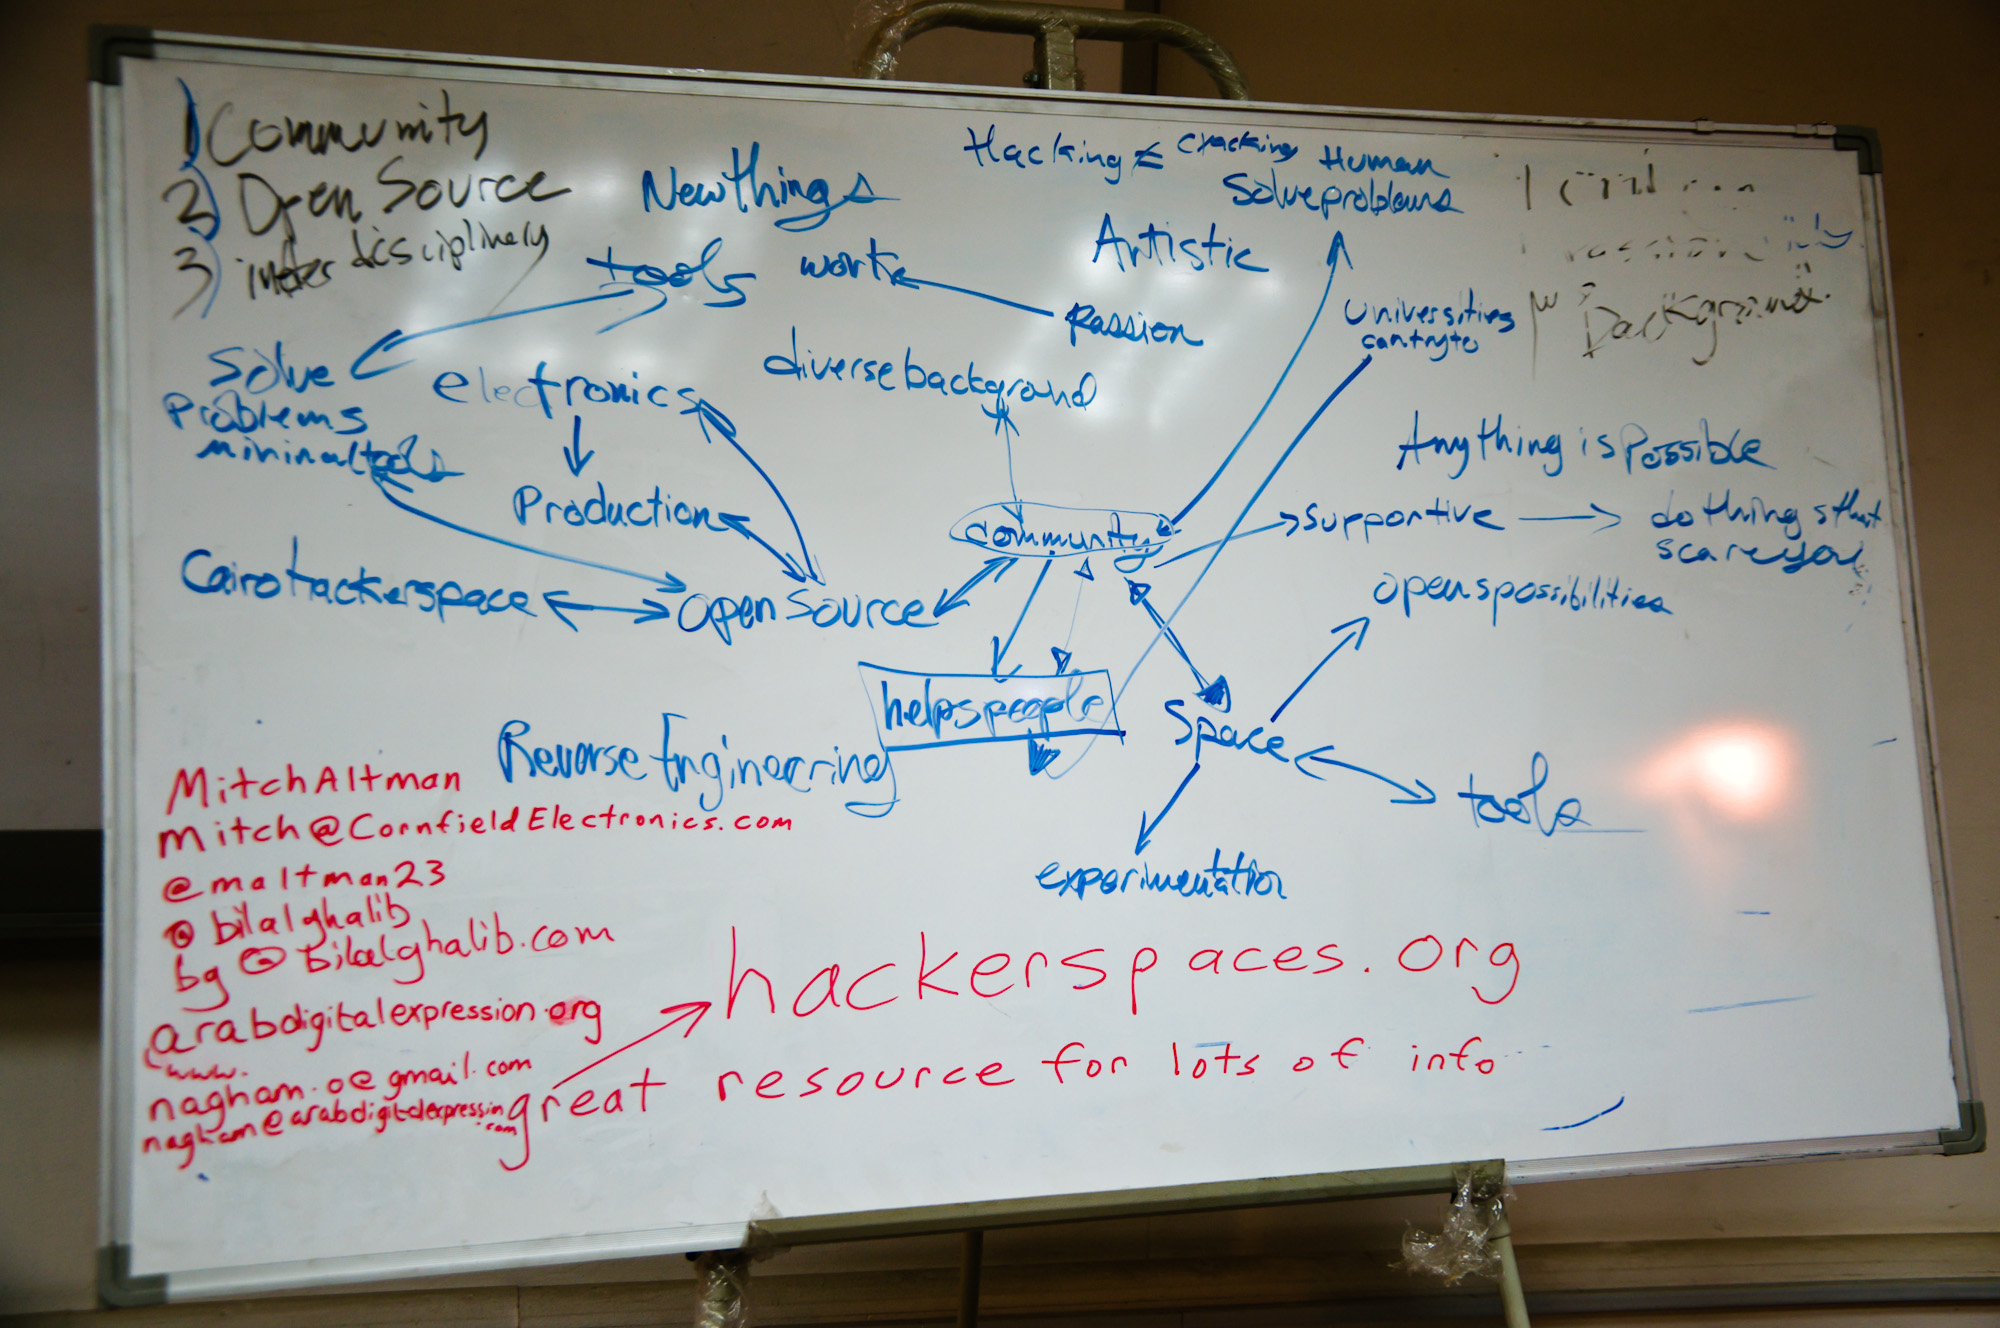
\includegraphics[width=\paperwidth]{hackerspaces-whiteboard.jpg}}
    \begin{frame}{\boxx{Ende}}
      \bigskip
      \bigskip
      \bigskip
      \bigskip
      \bigskip
      \bigskip
      \bigskip
      \bigskip
      \bigskip
      \boxx{
        Für mehr Informationen besucht \url{http://hackerspaces.org}
      }\\
      \boxx{
        \tiny{
          Diese Präsentation gibt’s unter einer freien Lizenz unter
        }
      }\\
      \boxx{
        \tiny{
          \url{https://github.com/nomaster/hackspace-design-patterns}
        }
      }
      
\includegraphics[width=30px]{cc-by-nc-sa.png}
      \\
      \boxx{
        \tiny{Mic \flq nomaster@chaosdorf.de\frq}
        \tiny{@nomaster auf identi.ca und Twitter}
      }
      \photoby{maltman23}{https://secure.flickr.com/photos/maltman23/6255298112/}{CC by-sa}
    \end{frame}
  }

\end{document}
